%%
%% This is file `sample-sigconf.tex',
%% generated with the docstrip utility.
%%
%% The original source files were:
%%
%% samples.dtx  (with options: `sigconf')
%% 
%% IMPORTANT NOTICE:
%% 
%% For the copyright see the source file.
%% 
%% Any modified versions of this file must be renamed
%% with new filenames distinct from sample-sigconf.tex.
%% 
%% For distribution of the original source see the terms
%% for copying and modification in the file samples.dtx.
%% 
%% This generated file may be distributed as long as the
%% original source files, as listed above, are part of the
%% same distribution. (The sources need not necessarily be
%% in the same archive or directory.)
%%
%%%% Proceedings format for most of ACM conferences (with the exceptions listed below) and all ICPS volumes.
\documentclass[sigconf, anonymous]{acmart}
\usepackage{cleveref}
\usepackage{graphicx}
\usepackage{subfigure}
\usepackage{threeparttable}
\usepackage{enumitem}
\usepackage{bigstrut,multirow}
\usepackage{algorithm}  
\usepackage{algorithmicx}  
\usepackage{algpseudocode}  
\usepackage{amsmath} 
\usepackage{lipsum}
% \floatname{algorithm}{ROSExample} 
%%%% As of March 2017, [siggraph] is no longer used. Please use sigconf (above) for SIGGRAPH conferences.

%%%% Proceedings format for SIGPLAN conferences 
% \documentclass[sigplan, anonymous, review]{acmart}

%%%% Proceedings format for SIGCHI conferences
% \documentclass[sigchi, review]{acmart}

%%%% To use the SIGCHI extended abstract template, please visit
% https://www.overleaf.com/read/zzzfqvkmrfzn

%%
%% \BibTeX command to typeset BibTeX logo in the docs
% \AtBeginDocument{%
%   \providecommand\BibTeX{{%
%     \normalfont B\kern-0.5em{\scshape i\kern-0.25em b}\kern-0.8em\TeX}}}

%% Rights management information.  This information is sent to you
%% when you complete the rights form.  These commands have SAMPLE
%% values in them; it is your responsibility as an author to replace
%% the commands and values with those provided to you when you
%% complete the rights form.
% \copyrightyear{2019}
% \acmYear{2019}
% \setcopyright{rightsretained}

%% These commands are for a PROCEEDINGS abstract or paper.
% \acmConference{SIGGRAPH '19 Talks}{July 28 - August 01, 2019}{Los Angeles, CA, USA}
% \acmDOI{10.1145/3306307.3328180}
% \acmISBN{978-1-4503-6317-4/19/07}
% \acmBooktitle{SIGGRAPH '19 Talks, 
%   July 28 - August 01, 2019, Los Angeles, CA}


%%
%% Submission ID.
%% Use this when submitting an article to a sponsored event. You'll
%% receive a unique submission ID from the organizers
%% of the event, and this ID should be used as the parameter to this command.
%%\acmSubmissionID{123-A56-BU3}
 
%%
%% The majority of ACM publications use numbered citations and
%% references.  The command \citestyle{authoryear} switches to the
%% "author year" style.
%%
%% If you are preparing content for an event
%% sponsored by ACM SIGGRAPH, you must use the "author year" style of
%% citations and references.
%% Uncommenting
%% the next command will enable that style.
%%\citestyle{acmauthoryear}

%%
%% end of the preamble, start of the body of the document source.


\settopmatter{printacmref=false} % Removes citation information below abstract
\renewcommand\footnotetextcopyrightpermission[1]{} % removes footnote with conference information in first column
\pagestyle{plain} % removes running headers

\begin{document}

%%
%% The "title" command has an optional parameter,
%% allowing the author to define a "short title" to be used in page headers.
% \title{MUROEXE : A Multi-Agent Exploration Engine Based on Interruptable CNN Accelerator on Embedded FPGA}
\title{INCAME : INterruptable CNN Accelerator for Multi-robot Exploration}

%%
%% The "author" command and its associated commands are used to define
%% the authors and their affiliations.
%% Of note is the shared affiliation of the first two authors, and the
%% "authornote" and "authornotemark" commands
%% used to denote shared contribution to the research.
\author{Jincheng Yu}
% \authornote{Both authors contributed equally to this research.}

%%
%% By default, the full list of authors will be used in the page
%% headers. Often, this list is too long, and will overlap
%% other information printed in the page headers. This command allows
%% the author to define a more concise list
%% of authors' names for this purpose.
% \renewcommand{\shortauthors}{Trovato and Tobin, et al.}

%%
%% The abstract is a short summary of the work to be presented in the
%% article.
\begin{abstract}
Multi-robot exploration (MR-Exploration) that provides the location and maps is the basic task for many multi-robot applications. 
With the development of Convolutional Neural Network (CNN), the accuracy of some critical components in MR-Exploration, such as Feature-point Extraction (FE) and Place Recognition (PR), can significantly benefit from CNN. 
To deploy CNNs on the embedded real-time system, previous works design CNN accelerators on FPGA. 
However, previous CNN accelerators mainly focused on improving the performance of a single neural network, lacking multi-task support.
Since researchers in robotics usually run different CNN tasks simultaneously, the inability of accelerators to support multi-task makes it difficult for researchers in robotics to use embedded FPGA.

We propose an INterruptible CNN Accelerator for Multi-robot Exploration (INCAME) for rapid deployment of MR-Exploration on FPGA.
INCAME proposes a virtual-instruction-based interrupt method to support multi-task on CNN accelerators.
After accelerating  CNN backbones, the post-processing of  CNN-based components (such as PR and FE), which is also computation consuming, becomes the bottleneck of the system.
Thus, INCAME also includes RTL/HLS hardware modules to accelerate the post-processing of the CNN-based components.
We evaluate INCAME on Xilinx ZU9 MPSoC. The experiment results show that INCAME enables multi-task scheduling on the CNN accelerator with negligible performance reduction (??\%). With the help of multi-task, INCAME enables embedded FPGA (Xilinx ZU9) executing MR-Exploration in real-time (20 fps).
% Multi-robot exploration (MR-Exploration) that provides the location and maps is the basic task for many multi-robot applications. 
% Feature-point Extraction (FE) and Place Recognition (PR) are two critical modules in MR-Exploration.
% The accuracy of both modules can benefit from Convolutional Neural Network (CNN).
% Previous CNN accelerators on FPGA mainly focus on improving the performance of a single neural network, lacking multi-task support.
% Researchers in robotics usually run several CNN tasks simultaneously, such as FE and PR.
% The inability of CNN accelerators to support multi-task makes it difficult for researchers in robotics to use embedded FPGA.

% We propose a \textit{MU}lti-\textit{RO}bot \textit{EX}ploration \textit{E}ngine (MUROEXE) to deploy MR-Exploration on embedded FPGA. 
% We propose a virtual-instruction-based interrupt method to support multi-task on CNN accelerators.
% Besides the CNN backbone, the post-precessing for CNN-based FE and PR is also computation consuming. 
% MUROEXE introduces RTL/HLS modules to accelerate the post-precessing of CNN-based modules.
% Experiments show that MUROEXE supports multi-thread scheduling with negligible performance reduction (??\%).
% MUROEXE enables embedded FPGA (Xilinx ZU9) executing MR-Exploration in real-time (30 fps).
\end{abstract}

%%
%% The code below is generated by the tool at http://dl.acm.org/ccs.cfm.
%% Please copy and paste the code instead of the example below.
%%
% \begin{CCSXML}
% <ccs2012>
%  <concept>
%   <concept_id>10010520.10010553.10010562</concept_id>
%   <concept_desc>Computer systems organization~Embedded systems</concept_desc>
%   <concept_significance>500</concept_significance>
%  </concept>
%  <concept>
%   <concept_id>10010520.10010575.10010755</concept_id>
%   <concept_desc>Computer systems organization~Redundancy</concept_desc>
%   <concept_significance>300</concept_significance>
%  </concept>
%  <concept>
%   <concept_id>10010520.10010553.10010554</concept_id>
%   <concept_desc>Computer systems organization~Robotics</concept_desc>
%   <concept_significance>100</concept_significance>
%  </concept>
%  <concept>
%   <concept_id>10003033.10003083.10003095</concept_id>
%   <concept_desc>Networks~Network reliability</concept_desc>
%   <concept_significance>100</concept_significance>
%  </concept>
% </ccs2012>
% \end{CCSXML}

% \ccsdesc[500]{Computer systems organization~Embedded systems}
% \ccsdesc[300]{Computer systems organization~Redundancy}
% \ccsdesc{Computer systems organization~Robotics}
% \ccsdesc[100]{Networks~Network reliability}

%%
%% Keywords. The author(s) should pick words that accurately describe
%% the work being presented. Separate the keywords with commas.
\keywords{FPGA, CNN accelerator, Multi-Robot}


%%
%% This command processes the author and affiliation and title
%% information and builds the first part of the formatted document.
\maketitle

\section{INTRODUCTION}
\label{sec:intro}

In recent years, with the development of hardware and algorithm, the intelligence of a single agent has been greatly improved.
The cooperation of agents can expand the capability of an unmanned system [??], and the multi-agent intelligent system is a promising research field.

Multi-robot exploration (MR-Explore) provides location and map for each robot. It is the basic task for many multi-robot applications, such as multi-robot navigation [??] and multi-robot rescue[??].

For the keyword \textit{"robot"}, the feature-point extraction (FE) is a fundamental component for the visual odometry to estimate the 6 degrees of freedom (6-DoF) pose [??].
For the keyword \textit{"multi"}, place recognition (PR) converts the input image into a short representation code, which is a fundamental element to produce candidate place matches between different robots [??].
Recent works use CNN to extract feature-points \cite{detone2018superpoint, simo2015discriminative, yi2016lift} and generate the representation code \cite{arandjelovic2016netvlad, radenovic2018fine}. 
The CNN-based feature-points from \cite{detone2018superpoint} reaches 10\%-30\% higher matching accuracy compared with the popular handcrafted extraction method, ORB \cite{Mur-Artal:2017281}.
The accuracy of the representation code from CNN-based method \cite{radenovic2018fine} is also ??\% better than the handcrafted method [??].

\begin{figure}[t]
	\centering
	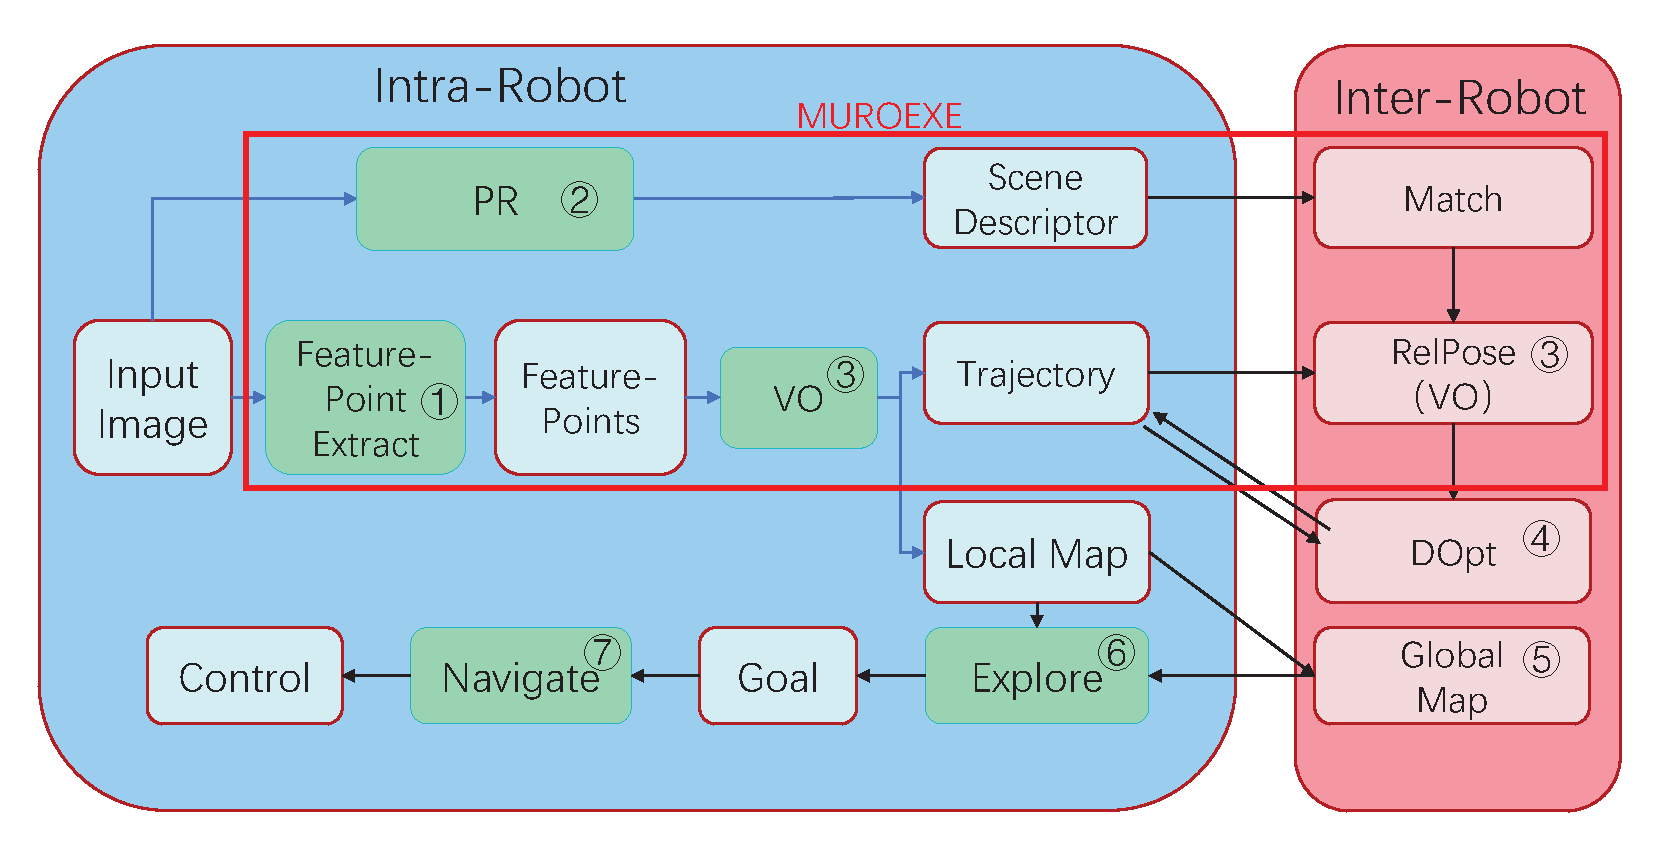
\includegraphics[width=0.99\linewidth]{fig/maexp.eps}
    \caption{
        The modules in MR-Explore. \textcircled{1}\textcircled{3} are basic for a single robot, should be execute every frame. \textcircled{2} generates representation code for some key frames. \textcircled{7}\textcircled{8} are only executed when representation codes are matched across robots and they are latency tolerant.  \textcircled{4}\textcircled{5}\textcircled{6} are for decision and navigation, also latency tolerant.
    }
	\label{fig:maexp}
\end{figure}


\Cref{fig:maexp} illustrates the computation modules in MR-Explore.
Feature-point extraction (\textcircled{1}) and visual odometry (VO, \textcircled{3}) should be performed for each input frame, and should be completed before the next frame. 
Place Recognition (PR, \textcircled{2}) generates the representation code for some key frames, and sends them to other robots. 
When the  representation codes from different robots are matched, optimization (\textcircled{7}) and map merging ((\textcircled{8})) are performed to merge the trajectories and maps. \textcircled{4}\textcircled{5}\textcircled{6} are for decision-making and navigation based on the merged maps. 
In this paper, CNN methods are used to realize the Feature-point Extraction (\textcircled{1}) and  Place Recognition (\textcircled{2}).
Besides these two modules, more CNN-based methods, such as semantic segmentation \cite{long2015fully} and object detection \cite{ren2015faster}, can be introduced into embedded moving robots to achieve better accuracy.
Even if only FE and PR are implemented in CNN, the computational complexity reaches 1 TOP/s , which poses a challenge for embedded systems.


\begin{figure*}[t]
    % \flushleft
    \centering
	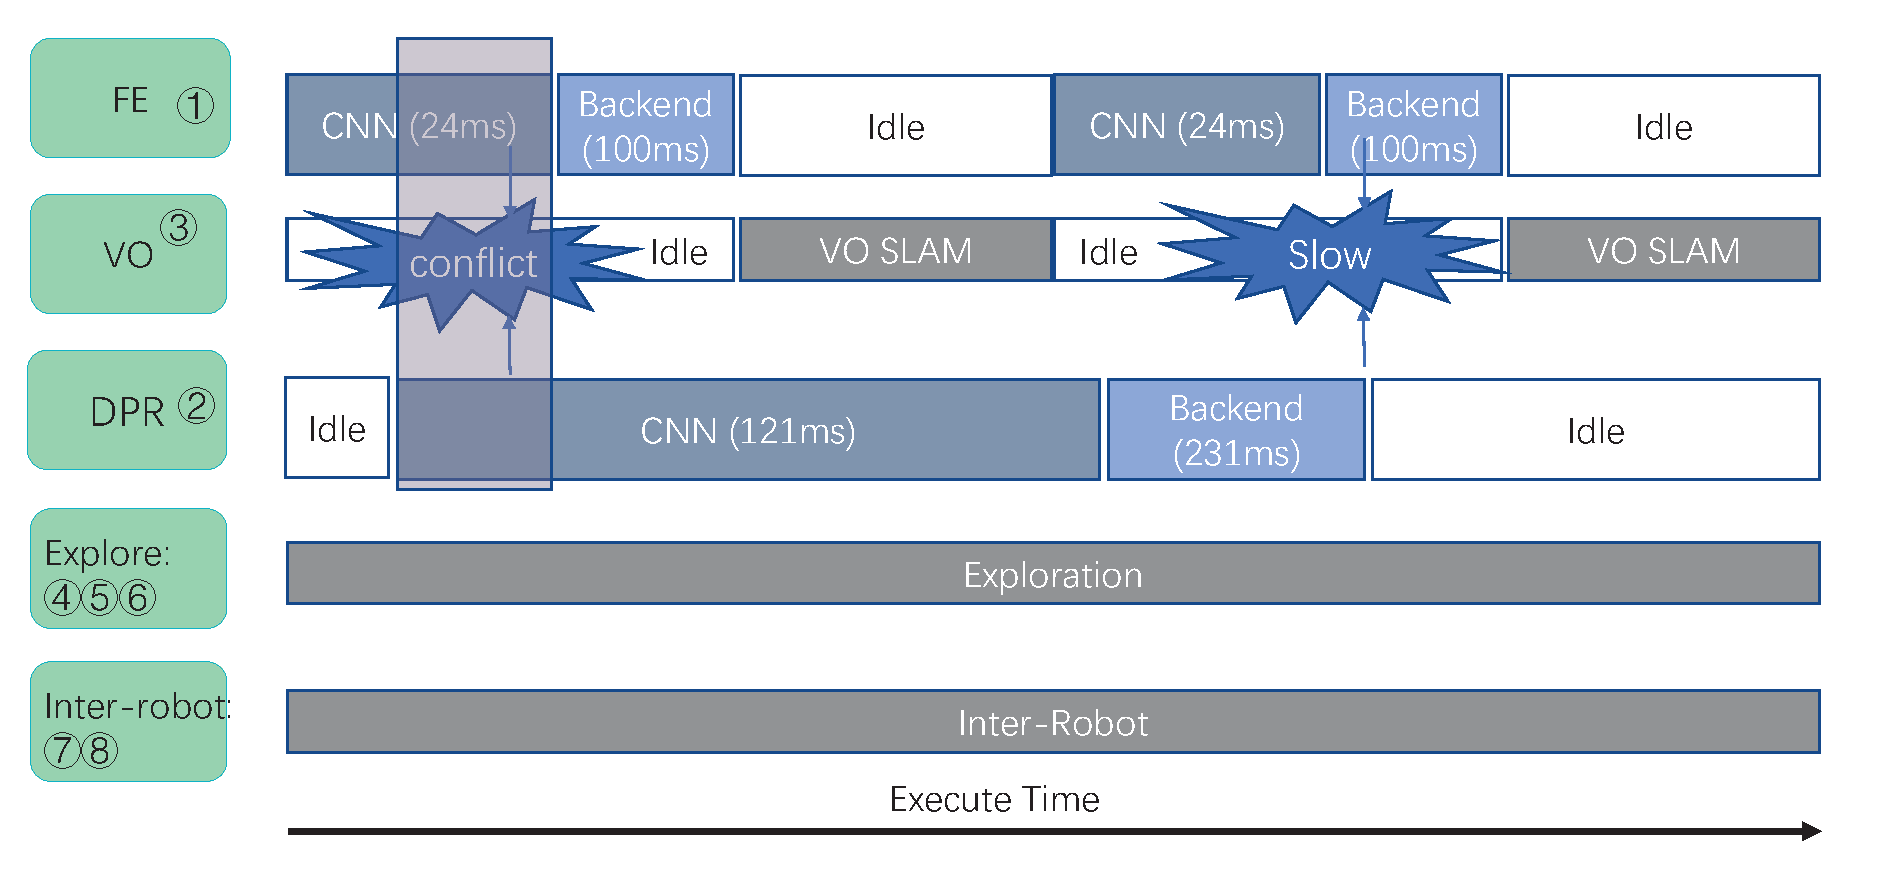
\includegraphics[width=0.95\textwidth]{fig/overalltime.eps} 	
    \caption{
    The overall timeline of MA-Explore.
    }
	\label{fig:overalltime}
\end{figure*}


In recent years, FPGA is becoming a promising platform for algorithm acceleration. Previous works design CNN accelerators on FPGA \cite{yu2018instruction,li_high_2016,qiu2016going,lu_evaluating_2017}. With the help of network quantization and data reuse, the speed of CNN accelerators on embedded FPGA reaches 3TOP/s \cite{lu_evaluating_2017}.
However, previous CNN accelerators are designed and optimized to accelerate a specific CNN. They can not automatically schedule two or more tasks simultaneously. 
The inability of CNN accelerators to support multi-task makes it difficult for researchers in robotics to use embedded FPGA.



The overall timeline of MA-Explore is illustrated in \Cref{fig:overalltime}. 
The threads of FE and PR may need to process CNN at the same time, resulting in hardware resource conflicts. 
In order to facilitate robotic researchers to run several CNN tasks simultaneously on the FPGA accelerators, the accelerator should support the following functions:

\textbf{Multi-thread:} A robot contains many modules including perception, decision-making, and control. 
The Robot Operating System (ROS) \cite{quigley2009ros} is a popular middleware fusing different modules from different developers. 
In ROS, each module is considered as an independent thread on CPU. 
Different threads should have easy access to the FPGA accelerator.

\textbf{Dynamic Scheduling:} The execution of CNN is depended on other operations, like VO module in \Cref{fig:overalltime}. 
These operations are running at CPU, and the execution time varies with the input data [??] (10ms - 50ms for VO). 
The accelerators cannot predict when to start a task. 
Therefore, the FPGA accelerator should be scheduled dynamically to support irregular task requests from the software.

\textbf{Scheduling by priority:} Each module has different priority. The control and perception tasks usually have higher priorities, while the priorities of long-term decision and optimization are lower \cite{RamsauerKLM17}. The critical tasks need to be arranged first on FPGA accelerators.

Besides the CNN backbone, the post-processing of the CNN-based methods, including normalization, softmax, rank, etc., is also computation consuming. As illustrated in \Cref{fig:overalltime}, the execution time of post-processing on embedded CPU (~100ms) exceeds that of CNN backbone on the accelerator (30ms), which becomes the bottleneck of the system.


In order to make the CNN accelerator flexible enough for robotic researchers to use, and speed up the post-processing of CNN-based method, we propose a \textit{MU}lti-\textit{RO}bot \textit{EX}ploration \textit{E}ngine ( MUROEXE ). MUROEXE can automatically deploy the MR-Explore on embedded FPGA, with following contributions:

\begin{itemize}[leftmargin = 10 pt]
\item We propose a CNN-based MA-Explore framework based on FPGA. The modules in MUROEXE is designed for ROS \cite{quigley2009ros}, so that the modules can be easily used in other applications.
\item We propose a \textbf{virtual-instruction-based} interrupt method to make the CNN accelerator support dynamic multi-thread scheduling by priority.
\item We optimize the data flow of the post-processing operations. RTL/HLS modules are designed for the optimized post-processing.
\end{itemize}

The rest of this article is organized as follows: \Cref{sec:relate} will introduce the related work. \Cref{sec:cnninterrupt} details the {virtual-instruction-based} interrupt. \Cref{sec:hardsoftcodesign} optimizes the post-processing. \Cref{sec:muroexe} introduces the MUROEXE framework with ROS. Experimental results and analysis are given in \Cref{sec:experiments}. \Cref{sec:conclusion} concludes this article.

\section{RELATED WORK}

\label{sec:relate}


\begin{figure*}[t]
	\centering
	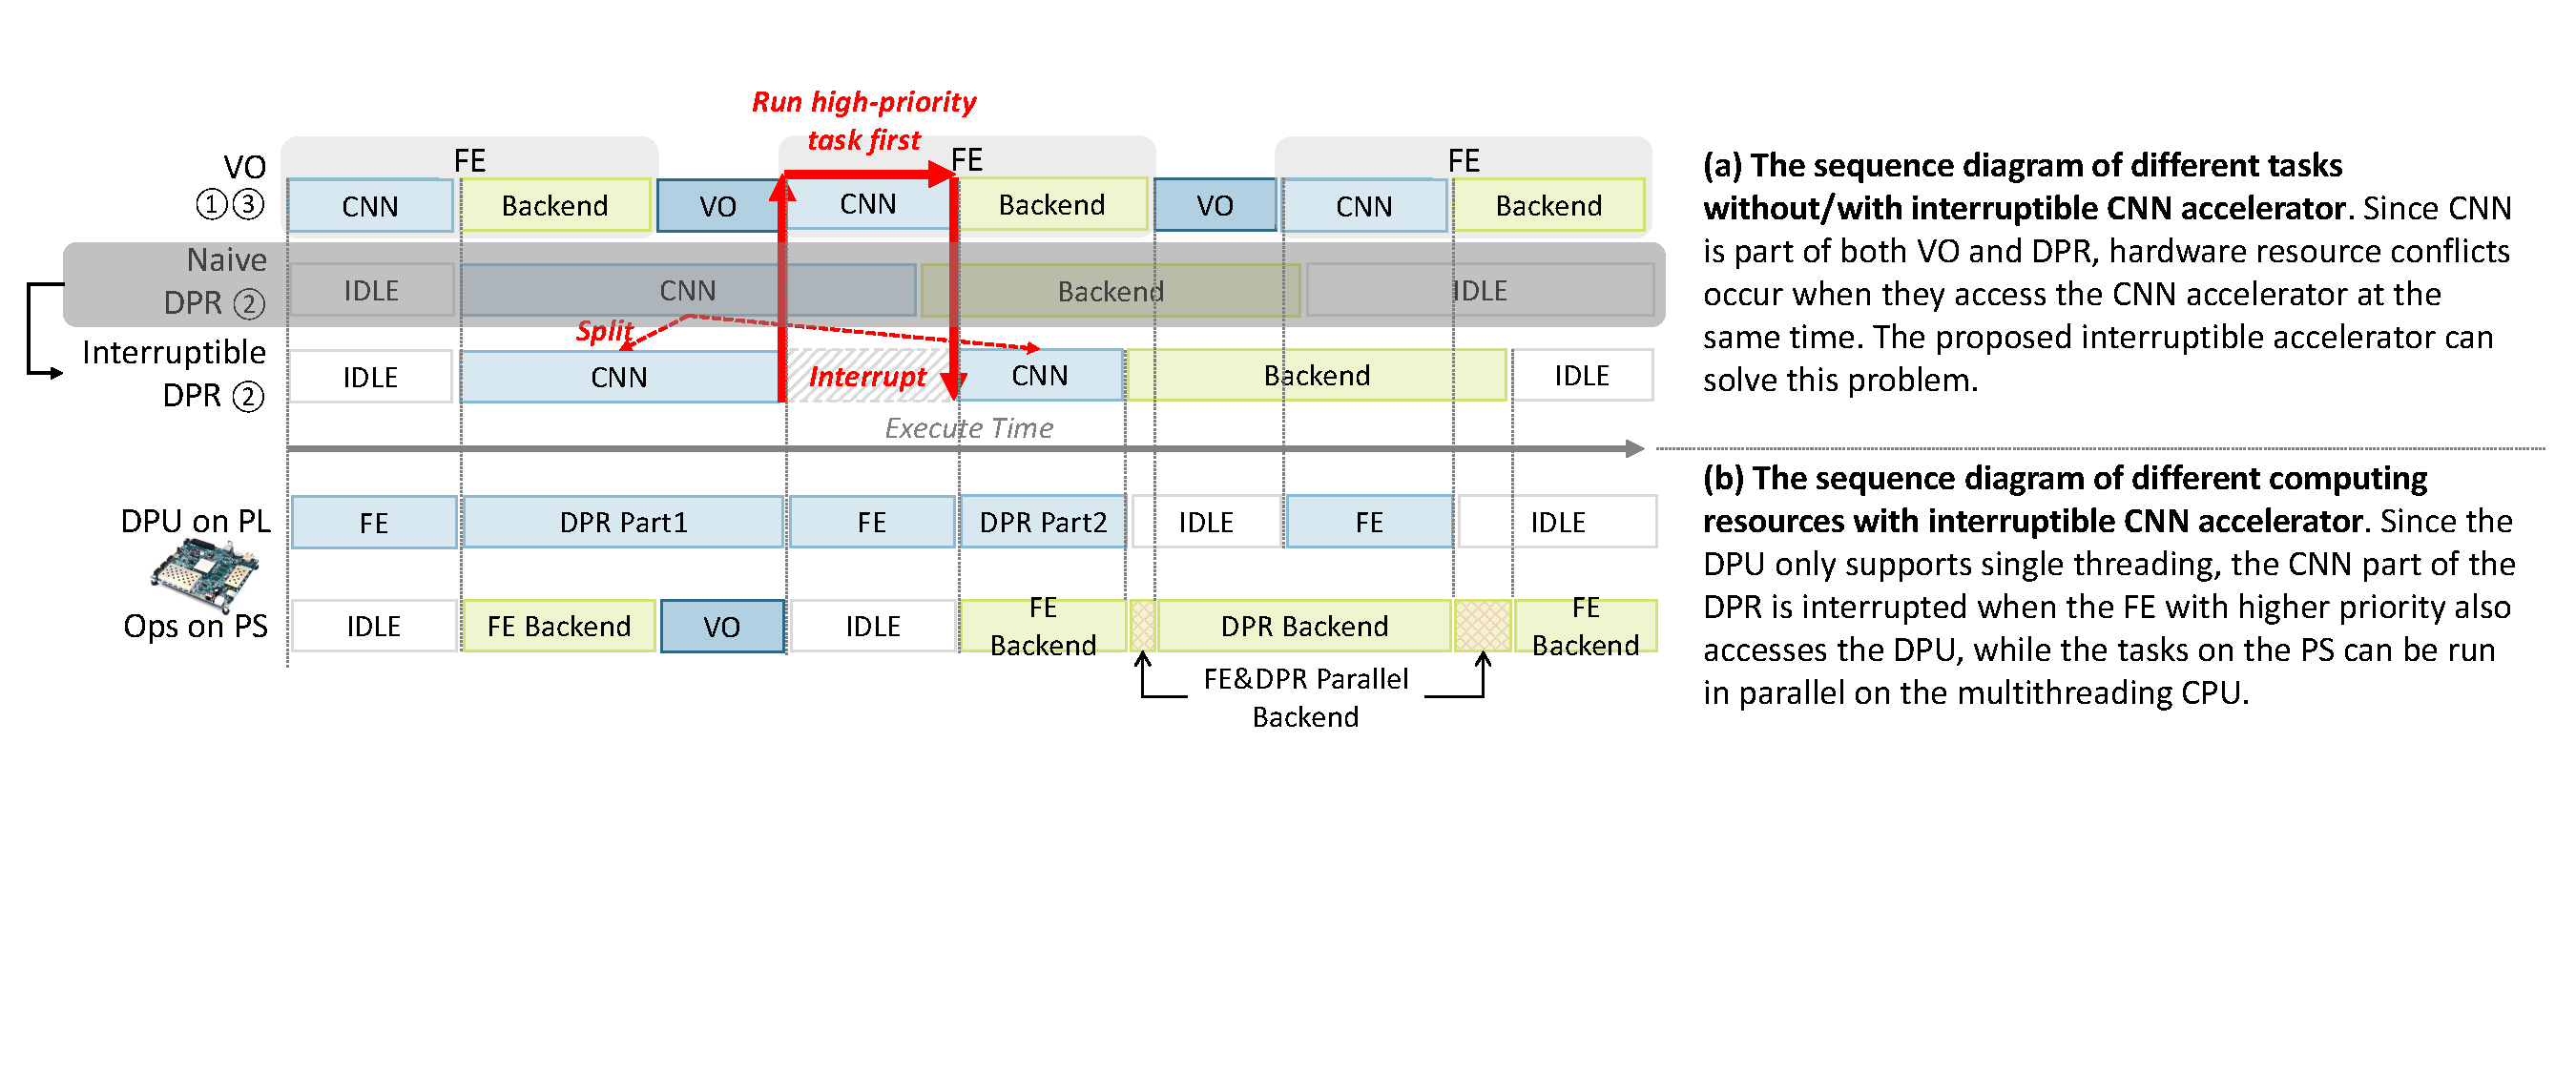
\includegraphics[width=0.99\linewidth]{fig/interDPR.pdf}
    \caption{Interruption to solve the hardware resources conflicts.  
    % When a high-priority task (FE) is started before the low-priority task (PR) is completed, the CNN accelerator backs up the status of PR to memory, and processes the FE task. When the high-priority task is completed, the low-priority task resumes and continues.
    }
	\label{fig:interDPR}
\end{figure*}


\subsection{ CNN-based FE and PR }

\textbf{\quad \ Feature-point extraction:} Previous feature-point extraction works usually consist of two parts: 1) feature-point detection to find the position of a feature-point and 2) descriptors generation to describe the extracted feature-point with a code.
SIFT \cite{lowe2004distinctive}  detects and describes the feature-points. The SIFT descriptor is rotation and scale invariant, so that the relative pose transformation between images with matching based on SIFT is accurate. However, the computaion of SIFT is complex and slow \cite{bay2006surf}. Thus, some other handcrafted method, such as SURF\cite{bay2006surf} and ORB \cite{Mur-Artal:2017281}, are proposed as fast alternatives to SIFT. ORB \cite{Mur-Artal:2017281} method are widely used for its balance between speed and accuracy.
Recently, CNN is used to extract feature-point. \cite{simo2015discriminative} proposes a CNN-based descriptor generator that exceeds ORB in accuracy.
DeTone \cite{detone2018superpoint} presents a fully CNN-based feature-point extraction method, SuperPoint, that implements feature-point detection and descriptors generation using one CNN network. SuperPoint\cite{detone2018superpoint} reaches 10\%-30\% higher matching accuracy compared the ORB based feature-point extraction \cite{Mur-Artal:2017281} and is used in this work.

\textbf{Place recognition:} Before CNN-based place recognition, Bag of Words (BoW) \cite{small_1} relying on handcrafted features is the most popular method. The accuracy of BoW-based methods is strongly influenced by the codebook size ( descriptor length ). Larger codebooks (~1M) \cite{large_1, large_2} can compete with CNN-based methods in accuracy. However, they take up huge storage and communication resources. Smaller codebooks\cite{small_1, small_2, jegou2014triang} require less space but get worse results. In contrast to traditional methods, CNN-based methods not only perform well but also generate more compact features, saving the storage and communication resources. GeM \cite{radenovic2018fine} and NetVLAD \cite{arandjelovic2016netvlad} are popular CNN-based methods, for their accuracy and data efficiency. GeM \cite{radenovic2018fine}, is also 20\% better than the handcrafted method rootSIFT \cite{jegou2014triang}.

Due to the advantage of CNN in image-based tasks, more and more CNN-based methods are used in the robot system.


\subsection{ FPGA accelerators for a specific robot task }

The feature-point extraction (FE) operation is the basic component of a visual-based robot, and is also one of the most time consuming components \cite{fang2017fpga}.
Some previous works design hardware architectures for FE.
SRI-SURF \cite{jia2016sri} optimizes the memory access to speed up SURF \cite{bay2006surf} feature-point extraction method. 
Fang \cite{fang2017fpga} directly implements ORB on FPGA using HLS. Liu \cite{liu2019eslam} optimizes the ORB algrithm and designs a hardware for better performance.
Some other works design architectures for the entire robot system. Hero \cite{shi2018hero} is a framework for navigation and laser-based robot and cannot support visual-based robots, which is much more lightweighted and cheaper. 
Li \cite{li2019879gops} introduces CNN accelerators for the visual-based robot
However, the CNN accelerator in this work\cite{li2019879gops} is only used for feature-point extraction, and the accelerator is not to support different tasks at the same time. 

Deploying multiple CNNs on robotic accelerator can expand the functions of robots, without designing hardware for a specific function.



\subsection{ CNN accelerators }

To accelerate CNN on FPGA, some previous works design frameworks to generate a specific hardware architecture for a target CNN, based on  RTL \cite{li_high_2016} or HLS \cite{lu_evaluating_2017}. These works need to reconfigure the FPGA to switch between different CNN models. The reconfiguration comsumes seconds \cite{FPGAPerformance}, which is unacceptable for the real time system.
Some other works design instruction-driven accelerators \cite{yu2018instruction,qiu2016going,guo2017angel}, making rapid switching possible by providing different instruction sequences. 
However, the CNN tasks on previous instruction-driven CNN accelerators are not interruptible, resulting in the latency-sensitive high-priority task waiting for the low-priority task to finish. 

This inability of CNN accelerators to support multi-task makes it difficult for robotics researchers to use embedded FPGA.

% However, previous instruction-driven CNN accelerators need to schedule the entire CNN, and can not automatically schedule two or more tasks simultaneously. The inability of CNN accelerators to support multi-task makes it difficult for robotics researchers to use embedded FPGA.

\section{INCAME Framework}
\label{sec:incame}

In this section, we firstly give a brief introduction to ROS\cite{quigley2009ros}. To solve the hardware resources conflicts in ROS, we propose the INCMAE framework for ROS softwares to access the CNN accelerator.




\subsection{Introduction to ROS}
Building a real robot requires many different components, including sensors, perception algorithms and control units from different developers. The Robot Operating System (ROS) \cite{quigley2009ros} is proposed to fuse the components from different researchers into a practical system. ROS is a popular framework for developing robot, which provides programming specifications and a communication interface. Node and Topic are the basic elements in ROS.

\textbf{Node.} Each function module in ROS, such as FE,PR,VO is called a node. Each node is an independent thead running on CPU, and  do not konw the running status of others.

\textbf{Topic.} Different nodes communicate with others by topics. A node can publish some topics and subscribe some topic. The publishing node is called publisher, the subscribing node is called subscriber.

\textbf{Publisher.} When the output of a publisher node is ready, the output data are inmediately packaged to the topic and published. ROS provides some system publisher, such as cv\_camera \cite{cvcamera} to read the camera and publish the input frames to a ROS topic.

\textbf{Subscriber.} The subscriber processes received topics through \textbf{callback} functions. Each callback function is bound to a topic. When the topic receives data, the callback function executed to process the data. If the callback function cannot complete before receiving the new data, the newly received data will be discarded.

The publisher and the subscriber are independent and communicate with each other only through topics. They do not even know if another one exists. 
The code examples in shown in \Cref{code:FE} and \Cref{code:PR}. line 17,18 in \Cref{code:FE} and line 12,13 in \Cref{code:PR} bind the topics with the callback functions.



Line 13 in \Cref{code:FE} and line 9 in \Cref{code:PR} initialize the accelerator for each task. Line5 in \Cref{code:FE} an d line 3 in ROSExample2 run the tasks on the same CNN accelerator respectively, which may result in hardware conflicts. 

\subsection{Hardware Resources Conflicts in ROS}

Although ROS is now becoming the fundamental software platform for robotics, the independence between different ROS nodes brings \textbf{hardware resources conflicts challenge} to access the hardware accelerator. 
Because developers cannot predict the running state of the CNN accelerator when they write programs, the accelerator may be occupied by other threads when a ROS node needs to call the accelerator. Line 13 in \Cref{code:FE} and line 9 in \Cref{code:PR} initialize the same accelerator for each task. Line5 in \Cref{code:FE} and line 3 in \Cref{code:PR} run the tasks on the same CNN accelerator, which may result in hardware conflicts.

To address this problem, we set the priorities of different tasks at the initialization phase (the {\color{red}priority} parameter in  \Cref{code:FE} line 13 and \Cref{code:PR} line 9 ), and enable the accelerator interrupt to schedule the high-priority task firstly.

% The run-time status of the CNN accelerator is not predictable when developers writing the program. Line 13 in ROSExample1 and line 9 in ROSExample2 initialize the DPU for each task. Line5 in ROSExample1 an d line 3 in ROSExample2 run the tasks on the same CNN accelerator, which may result in hardware conflicts. In INCAME, the priorities of different tasks are configured at initialization phase to address the hardware conflicts problem.


\begin{algorithm}[h]
    \caption{ ROS Node for FE }
    \label{code:FE}
    \begin{algorithmic}[1]
        \State {\color{gray} // imagePtr, imageAddr, fmPtr, fmAddr, DPUtask, Bankendtask  is initialized by main and used in FEcallback.}
        \Function {FEcallback}{$ InputFrame $}
        \State {\color{gray} // Read and reshape the InputFrame. }
        \State {\color{blue} *imagePtr  $\gets$ *InputFrame }
        \State DPUtask.run()
        \State FEBackend.run()
        \EndFunction

        \Function {Main}{$ $}
        \State {\color{gray} // Init ScratchPad Memory. Ptr is for CPU operations, Addr is for FPGA modules.}
        \State imagePtr, imageAddr = ScratchPad(FEinputsize)
        \State fmPtr, fmAddr = ScratchPad(FEfmsize)
        \State {\color{gray}// Config task0 in IAU of the accelerator (DPU).}
        \State DPUtask = DPUinit({\color{red}  priority=0},{\color{blue} instraddr=FEinstrAddr, }
        \State \qquad \qquad \qquad \quad {\color{blue} inoffset=imageAddr,outoffset=fmAddr } ) 
        \State FEBackend = FEBackendinit({\color{blue}fmAddr, fmPtr});
        \State {\color{gray}// The node subscribes the inputframe, and use the FEcallback to process each inputframe.}
        \State Subscriber = Node.subscribe( InputFrameTopic, FEcallback);
        \State {\color{gray}// Use spin to start the subscriber}
        \State Subscriber.spin();
        \EndFunction
    \end{algorithmic}
\end{algorithm}

\begin{algorithm}[h]
    \caption{ ROS Node for PR }
    \label{code:PR}
    \begin{algorithmic}[1]
        \Function {PRcallback}{$ InputKeyFrame $}
        \State {\color{blue} *imagePtr  $\gets$ *InputKeyFrame }
        \State DPUtask.run()
        \State PRBackend.run()
        \EndFunction

        \Function {Main}{$ $}
        \State imagePtr, imageAddr = ScratchPad(PRinputsize)
        \State fmPtr, fmAddr = ScratchPad(PRfmsize)
        \State DPUtask = PR\_DPUinit( {\color{red} priority=1},{\color{blue} instraddr=PRinstrAddr}, 
        \State \qquad \qquad \qquad \quad {\color{blue} inoffset=imageAddr,outoffset=fmAddr } ) 
        \State PRBackend = PRBackendinit({\color{blue}fmAddr, fmPtr});
        \State Subscriber = Node.subscribe( InputKeyFrameTopic, PRcallback);
        \State Subscriber.spin();
        \EndFunction
    \end{algorithmic}
\end{algorithm}

\subsection{ Accelerator interrupt to solve Hardware Resources Conflicts }

In order to support multi-task scheduling and solve the hardware resources conflicts, interrupt is introduced in CPU \cite{jen1974processor}. 


% If the CNN accelerator supports interrupt, it can run two or more CNN modules at the same time. 
\Cref{fig:interDPR} illustrates the idea of interrupt to schedule two CNN tasks. In the process of running a low-priority network (PR), the software may send an execution request for the high-priority task (FE). The interrupt enables the CNN accelerator to backup the running state of previous task low-priority PR network, and then execute the high-priority FE network. When the high-priority task (FE) is complete, the low-priority task (PR) is restored to the accelerator and continues to execute.
With the help of accelerator interrupt, the execution of the low-priority task (PR) is divided into pieces, and each piece is allocated to the time interval of running the high-priority networks (FE). 
Accelerator interrupt multiplexes the time division of the accelerator, reduces the idle time of the accelerator, and improves the utilization of hardware resources. 


\begin{figure*}[t]
	\centering
    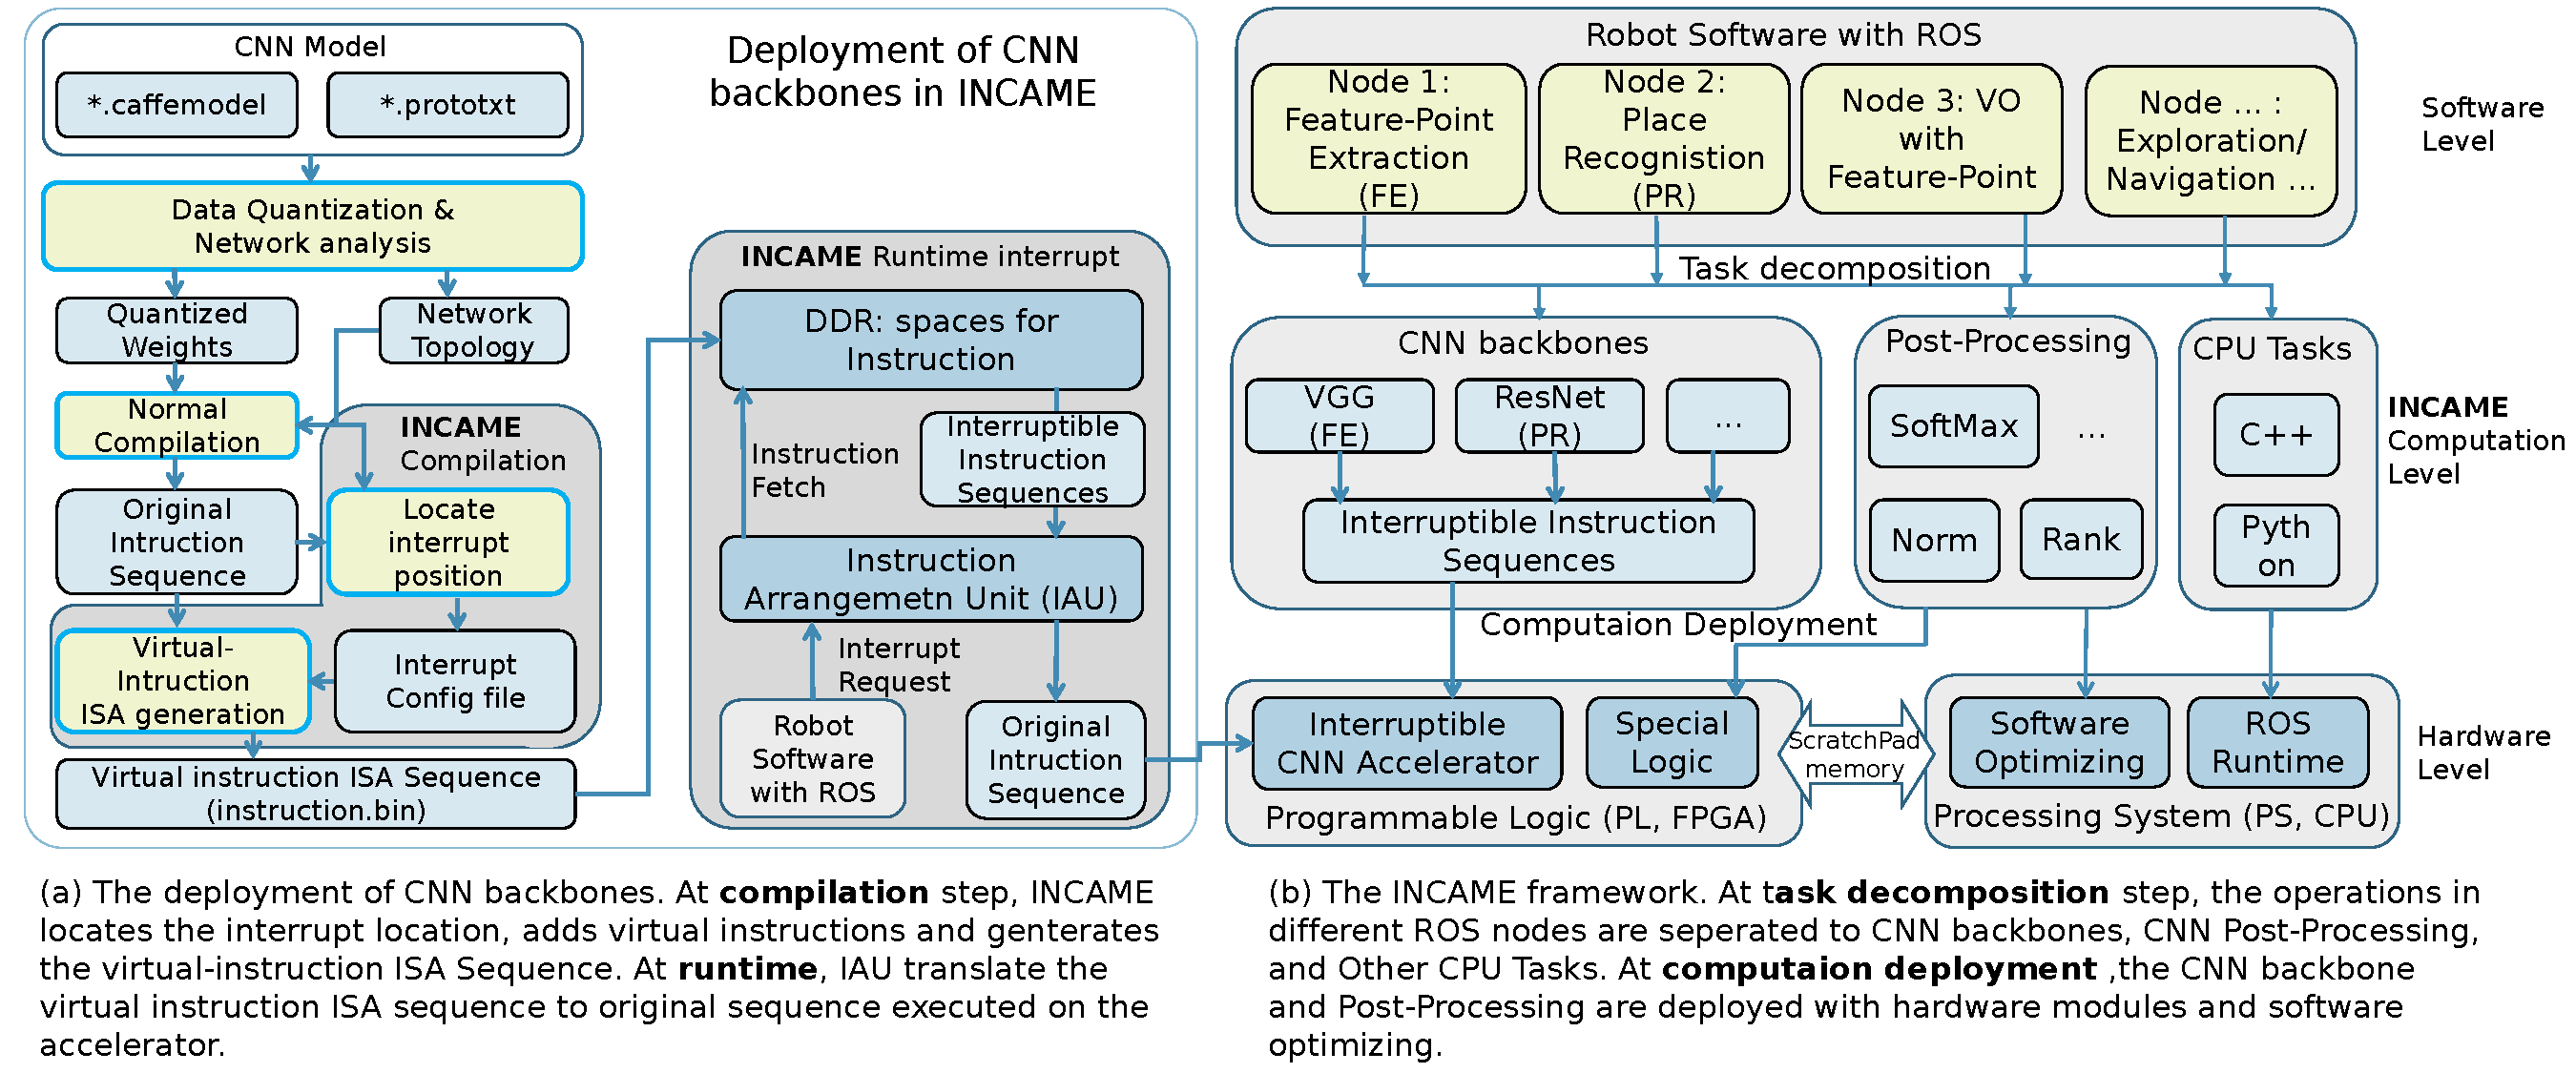
\includegraphics[width=0.99\linewidth]{fig/incame.pdf}
    \caption{ INCAME framework.}
	\label{fig:incame}
\end{figure*}

\subsection{ Interruptible Accelerator with ROS (INCAME) }

% We try to use CNN as much as possible to accomplish various tasks on the robot. Because the CNN not only has advantages over traditional algorithms in accuracy, but also has uniform and regular computing mode. Therefore, a single instruction-driven CNN accelerator can speed up different tasks. The unified accelerator can reduce the use of hardware resources and make it easier to implement the robot computing system on embedded FPGA.

\Cref{fig:incame}(b) illustrates the proposed two-step INCAME framework to mapping ROS based softwares to embedded FPGA.
The first step is the task decomposition, which decomposes the computation in ROS nodes into different INCAME computation types, including CNN backbones, CNN post-processing, and other CPU tasks. 

The second step is to deploy different computation on FPGA. 
The CNN backbones of  different task, such as the VGG model [??] in SupoerPoint feature-point extraction \cite{detone2018superpoint} and the ResNet101 model \cite{he2016deep} in GEM place recognition \cite{radenovic2018fine}, are compiled to the interruptible virtual-instruction instruction set architecture (VI-ISA). 
The interruptible CNN accelerator runs the instructions.
To accelerate the post-processing operations of the CNN based methods, hardware modules are implemented for the CPU-intensive Softmax and Normalization operations [??]. Some task-related software optimizations, such as Ranking and NMS [??], are processed in the CPU side of the embedded MPSoC\cite{MPSoC}.
Other tasks written in C++/Python run directly also on the CPU side.

To eliminate the memory copy between CPU cores and CNN accelerators, we use low-latency ScratchPad memory \cite{Banakar2002Scratchpad} to directly feed the results from CNN backbones to the post-processing modules. Each shared date in ScratchPad memory is initialized with two handlers: 1) a pointer (Ptr) for the CPU thread and 2) the physical address for the hardware modules. Blue lines in  ROSExample 1,2 illustrate the usage for the ScratchPad memory.

\Cref{fig:incame}(a) details the INCAME compilation step and runtime interrupt. Caffe [??] is a popular software framework for CNN, and the *.caffemodel/*.prototxt files define the network parameters and structure in Caffe. The pervious network deploy flow in Angel-Eye \cite{guo2017angel} quantizes the weights, and analysis the network topology. The original compiler in Angel-Eye translates the network topology and the quantization infomation into the original ISA sequence. INCAME compiler goes further than Angel-Eye. It select the optimized interrupt position in the original instruction flow, and adds virtual instructions at the interruptible position to enable accelerator interrupt. After that, the original instruction sequence and the added virtual instructions are wrapped to the new interruptible Virtual-Intruction ISA (VI-ISA). The wrapped VI-ISA instructions are dumped into a file (instruction.bin), and can be loaded into the instruction spaces on FPGA's DDR.

At runtime, an instruction arrangement unit (IAU) in hardware listens to the interrupt request from softwares, fetches the corresponding VI-ISA interruptible instructions and translates them to the original ISA executed on the CNN accelerator. 

The detail of the Virtual-Instruction ISA (VI-ISA) and instruction arrangement unit (IAU) is introduced in \Cref{sec:cnninterrupt}.

\section{Virtual-instruction-based Accelerator Interrupt}
\label{sec:cnninterrupt}
% The idea of interruption is introduced for dynamic multi-task scheduling. This section details the implementation of our \textbf{Virtual instruction Interruption}. \Cref{fig:interDPR} illustrates the idea of interruption to full utilize the hardware resources.

\begin{table*}[t]
	\footnotesize
	\centering
	\caption{Description for the basic instructions.}
% Table generated by Excel2LaTeX from sheet 'Sheet3'
\begin{tabular}{|p{2.7em}|p{3.4em}|p{16em}|p{4.2em}|p{4.6em}|p{4.2em}|p{4.2em}||p{7em}|p{7em}|}
	\hline
	\multicolumn{1}{|c|}{Category} & \multicolumn{1}{c|}{Type} & \multicolumn{1}{c|}{Description} & \multicolumn{1}{c|}{Address 1} & \multicolumn{1}{c|}{Address 2} & \multicolumn{1}{c|}{Address 3} & \multicolumn{1}{c||}{Workload} & \multicolumn{1}{c|}{Backups} & \multicolumn{1}{c|}{Recovery $^1$} \bigstrut\\
	\hline
	\multirow{2}[4]{*}{LOAD} & LOAD\_W & Load weights/bias from DDR to on chip weight buffer. & Off-chip Addr & Weights-buffer Addr & -     & Data  Length & -     & Weight / Inputdata \bigstrut\\
	\cline{2-9}\multicolumn{1}{|c|}{} & LOAD\_D & Load input data from DDR to on-chip data buffer. & Off-chip Addr & Data-buffer Addr & -     & Data  Length & -     & Weight / Inputdata \bigstrut\\
	\hline
	\multirow{2}[4]{*}{CALC} & CALC\_I & Calculate intermediate results for some output channels from partial  input channels. & Input  Data Addr & Intermediate Data Addr & Weight Addr & Calc Size & Previous final results / Intemediate data  & Weight / Inputdata /  intemediate data \bigstrut\\
	\cline{2-9}\multicolumn{1}{|c|}{} & CALC\_F & Calculate the results for some output channels from all input channels. The pooling, bias-adding and elementwise operations are operated in this instructions. & Input  Data Addr & Output  Data Addr & Weight Addr & Calc Size & Finial results & Weight / Inputdata \bigstrut\\
	\hline
	SAVE  & SAVE  & Save the results from on-chip data buffer to DDR. & Off-chip Addr & Data-buffer Addr & -     & Data  Length & -     & Weight / Inputdata \bigstrut\\
	\hline
	\end{tabular}%
	
	\label{tab:instr}%
  \end{table*}%


% \begin{figure*}[t]
% 	\centering
% 	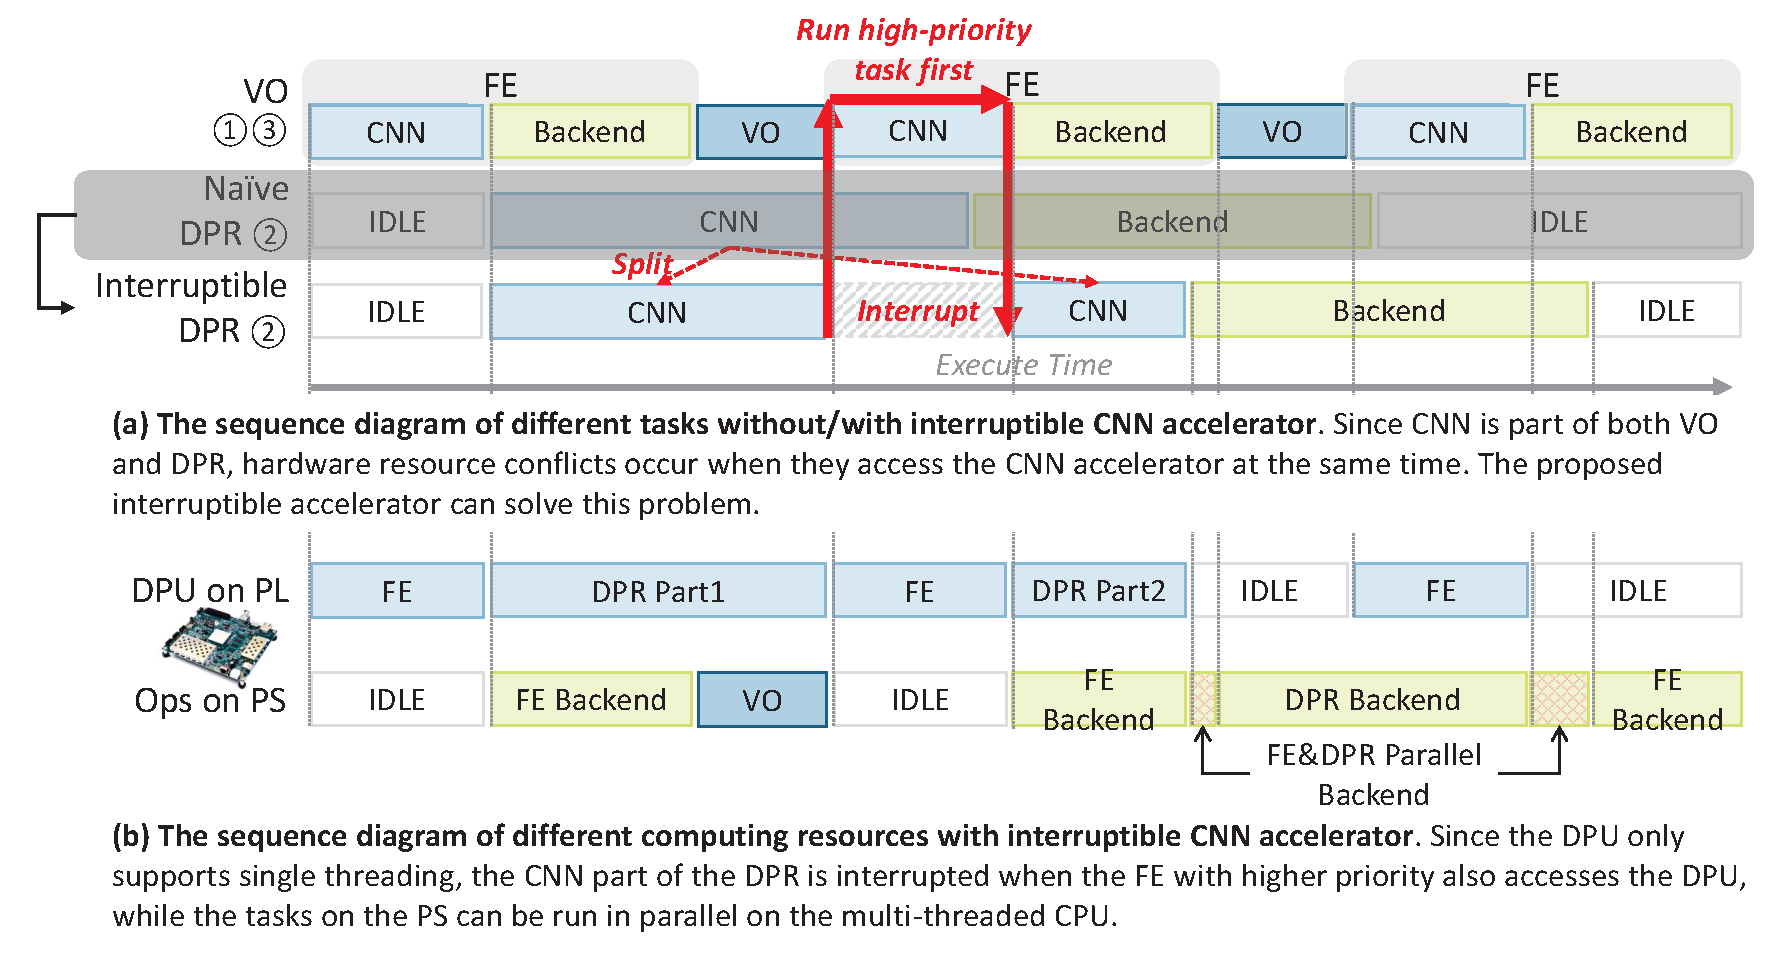
\includegraphics[width=0.9\linewidth]{fig/interDPR.eps}
% 	\caption{Interruption to solve the hardware resources conflicts.  When a high-priority task (FE) is started before the low-priority task (PR) is completed, the CNN accelerator backs up the status of PR to memory, and processes the FE task. When the high-priority task is completed, the low-priority task resumes and continues.
%     }
% 	\label{fig:interDPR}
% \end{figure*}

In this section, we introduce the concept of interrupt to CNN accelerator to support multi-task execution.

\subsection{Accelerator Interrupt}

In order to support multi-task scheduling, interrupt is introduced in CPU. 
In CPU, when a high-priority task requires an interrupt, the hardware or the interrupt handler software would back up the registers to main memory.
After the high-priority task is completed, the backed-up registers will be recovered to CPU hardware. 

If the CNN accelerator support interrupt, it can run two or more CNN modules at the same time. \Cref{fig:interDPR} illustrates the idea of interrupt to schedule two CNN tasks simultaneously. In the process of running a low-priority network (PR), the software may send an execution request for the high-priority task (FE). The interrupt enables the CNN accelerator to backup the running state of previous task low-priority PR network, and then execute the high-priority FE network. When the high-priority task (FE) is complete, the low-priority task (PR) is restored to the accelerator and continues to execute.

With the help of accelerator interrupt, the execution of the low-priority task (PR) is divided into pieces, and each piece is allocated to the time interval of running the high-priority networks (FE). 
Accelerator interrupt multiplexes the time division of the accelerator, reduces the idle time of the accelerator, and improves the utilization of hardware resources. 

\subsection{How To Interrupt: Virtual Instruction}
\label{sec:howinter}


However, the CPU-like interrupt would back up all the on-chip registers to DDR. In CPU, there are tens of registers, and the backed-up data is around 1 KB. In CNN accelerators, there are hundreds of KB ~ several MB on-chip cache \cite{qiu2016going, yu2018instruction}. If all the on-chip cache is backed-up and recovered, the cost of data transfer in the CNN accelerator is much higher than that of CPU.

We propose the \textbf{virtual-instruction-base} method to enable interrupt. The low-priority task maintains the executing status itself, rather than the hardware or the interrupt handler used in CPU. Only the cache which is still needed in future execution will be backed-up and restored.

The virtual instructions, which contain the backup and recovery instructions, are generated in the compilation phase, together with the normal instructions. 
For backup instructions, the corresponding input data and weights are still stored in DDR. 
There is no need to back up the input buffer and weight buffer, and only the intermediate data and the final output results are needed to be backed-up. 
For recovery instructions, the weights and input data for future calculation, as well as the backed-up intermediate data, are needed to be restored from DDR to the on-chip cache.

There is a field in the instruction set, that indicates whether the instruction a virtual instruction. If no interrupt occurs, virtual instructions will be skipped and discarded, which can ensure the efficiency of uninterrupted execution.

\subsection{ Where To Interrupt: After Save/CALC\_F }
\label{sec:whereinter}

There are three categories of instruction in the instruction-driven accelerator: LOAD, CALC, and SAVE. The instruction description and the backup/recovery data for interrupt position at each kind of instruction are listed in \Cref{fig:normal_instr} and \Cref{tab:instr}.

\begin{figure}[h]
	\centering
	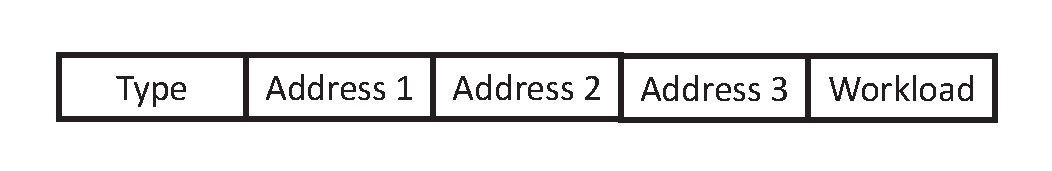
\includegraphics[width=0.9\linewidth]{fig/normal_instr.eps}
	\caption{The extended instruction set for virtual instruction }
	\label{fig:normal_instr}
\end{figure}



\subsubsection{LOAD\_W / LOAD\_D }
When an interruption occurs at LOAD, the newly loaded data would immediately be flushed when running the high-level CNN, leading to bandwidth waste.

\subsubsection{CALC\_I} 
When an interrupt occurs at CALC\_I, the unsaved finial results ( generated by previous CALC\_F) should be saved to DDR. The intermediate data from current CALC\_I should also be sent to DDR for further use. At the Recovery stage, the intermediate data should be fetched from DDR. The data movement of intermediate results leads to additional bandwidth requirements.


\subsubsection{CALC\_F}
When an interrupt occurs at CALC\_F, there is no need to back up and recovery intermediate results. Although it is necessary to back up the unstored final results which are generated by previous CALC\_F, these results will be stored in DDR through the subsequent normal SAVE instruction.
If the accelerator can record the interrupt status, we can modify the address and workload when executing subsequent normal not-virtual save instruction.
In this way, we can avoid the repetitive transmission of results.
The state records and modifications to normal SAVE instruction will be introduced in the following subsections.

\begin{figure}[h]
	\centering
	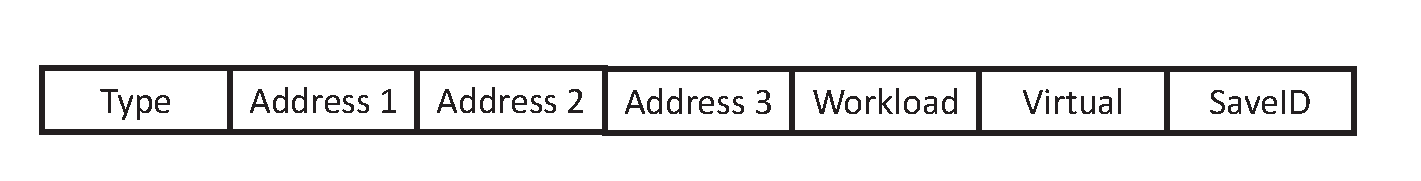
\includegraphics[width=0.99\linewidth]{fig/virtual_instr.eps}
	\caption{The basic structure of a instruction }
	\label{fig:virtual_instr}
\end{figure}



\begin{figure*}[t]
	\begin{minipage}[t]{0.49\linewidth}  
	\centering
	\subfigure[One Save for Single CACL/LOAD.] {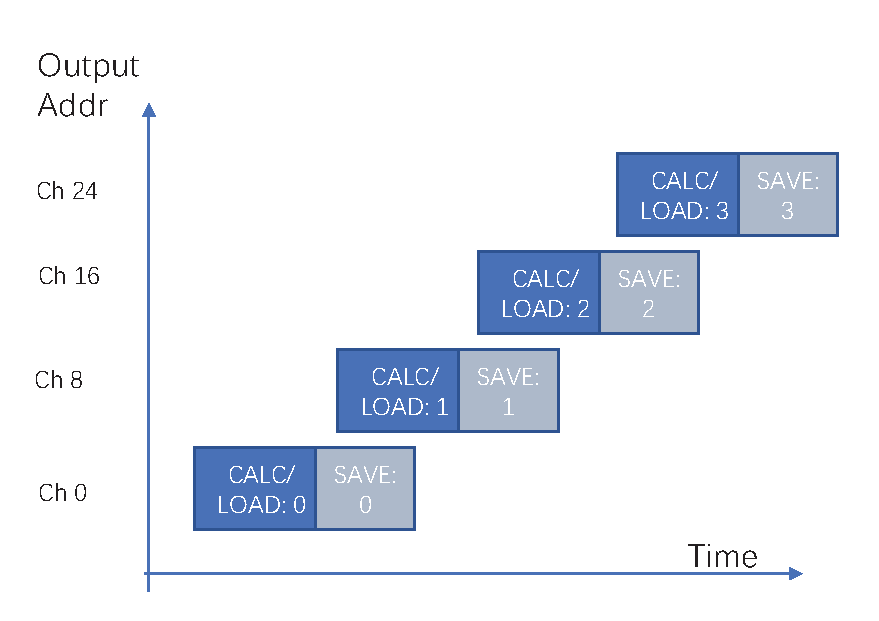
\includegraphics[width=0.9\linewidth]{fig/singlesave.eps}\label{fig:singlesave}}
	\end{minipage}
	\begin{minipage}[t]{0.49\linewidth}  
	\centering  
	\subfigure[One Save for Multiple CACL/LOAD.] {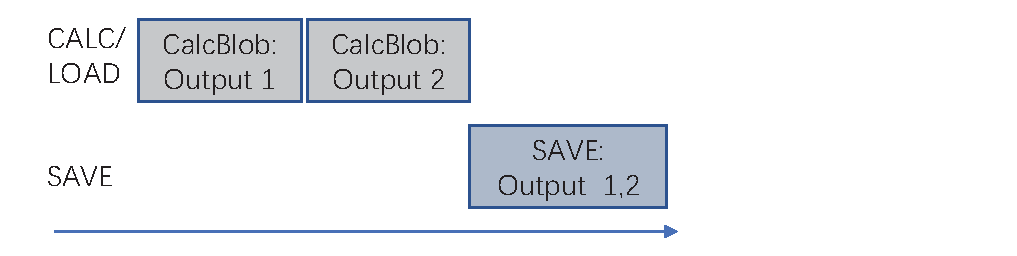
\includegraphics[width=0.9\linewidth]{fig/multisave.eps}\label{fig:multisave}} 

	\end{minipage}
	\begin{minipage}[t]{0.49\linewidth}  
	\centering  
	\subfigure[Interrupt for \Cref{fig:singlesave} ] {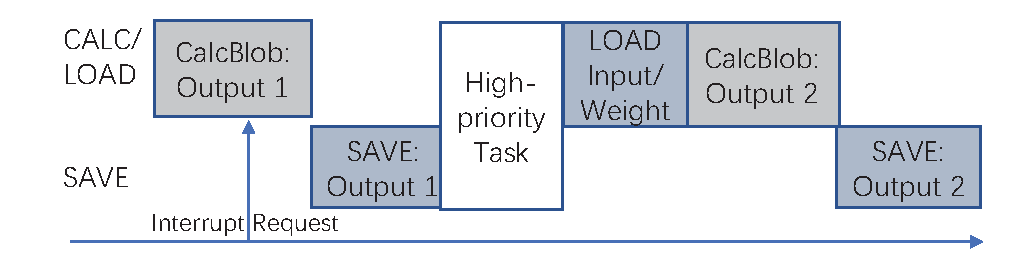
\includegraphics[width=0.9\linewidth]{fig/intersingle.eps}\label{fig:intersinglesave}} 
	\end{minipage}
	\begin{minipage}[t]{0.49\linewidth}  
	\centering  
	\subfigure[Interrupt for \Cref{fig:multisave}] {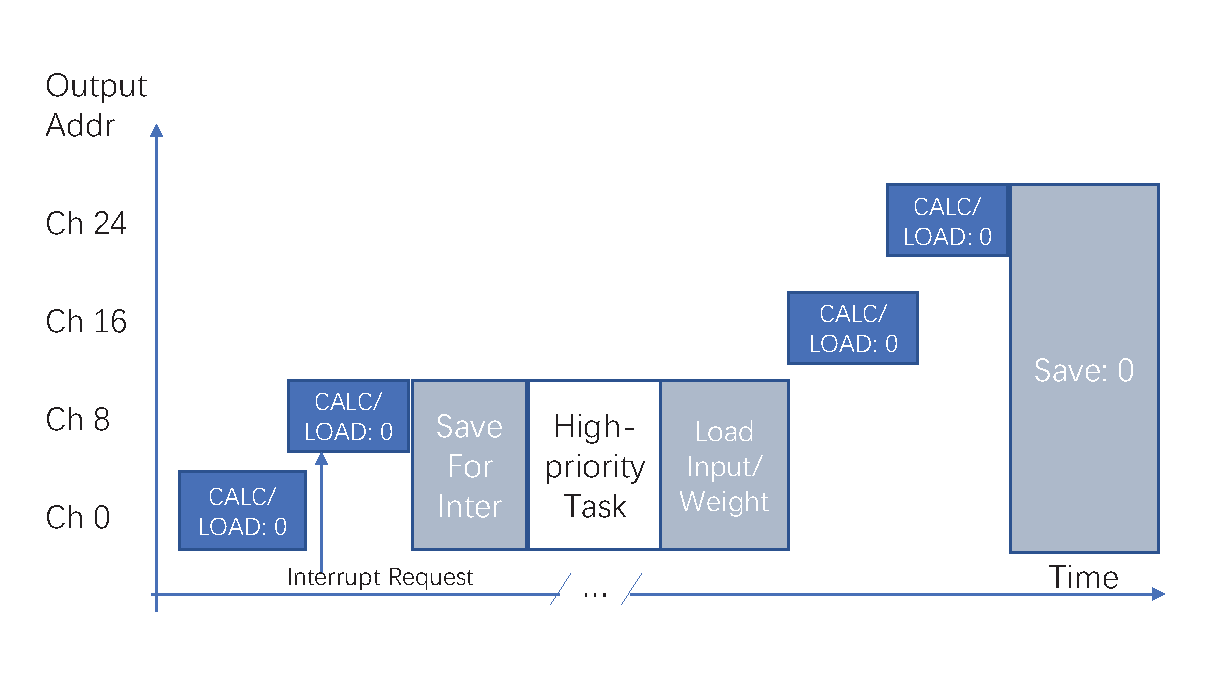
\includegraphics[width=0.9\linewidth]{fig/intermulti.eps}\label{fig:intermultisave}} 
	\end{minipage}
	\caption{ Scheduling Illustration
%   (d) find a single intra-robot loop closure which (c) and (d) cannot find, so that the result is better than (c) and (e).
  }
\label{fig:dslamresult}
\end{figure*}


\begin{figure}[t]
	\centering
	\includegraphics[width=0.99\linewidth]{fig/IAU.eps}
	\caption{Hardware Architecture of IAU. The software on the CPU side (PS side) communicates IAU to access the CNN accelerator. IAU records the running state of each task, such as the address to fetch instructions, the SaveID of interrupted instructions. At runtime, IAU translates the input instruction sequence with virtual instructions to a normal sequence of instructions. }
	\label{fig:IAU}
\end{figure}

\subsubsection{SAVE}
When an interrupt occurs at SAVE, there is no need to back up any data. The overhead of this interrupt is only to transfer input data and weights from DDR to the on-chip cache.

We want to minimize the cost of interrupt. We make the low-priority CNN interruptible after the SAVE or CACL\_F instructions. This method only introduces extra data transfer to recovery input data and weights without any excess backup data transfer.

Additional virtual instructions also take up bandwidth at instruction fetching phase, even if they are not executed. The instruction number of CALC\_I is tens of times of that of SAVE/CALC\_F. If the network can be interrupted after each CALC\_I, the rapidly increasing virtual instructions would reduce the system performance.

\subsection{ Instruction Set Improvement }
\label{sec:virtualinstr}

We extend the instruction set shown in \Cref{fig:normal_instr}. Two fields are added: 1) Virtual and 2) SaveID, as illustrated in \Cref{fig:virtual_instr}.

\begin{figure*}[t]
	\centering
	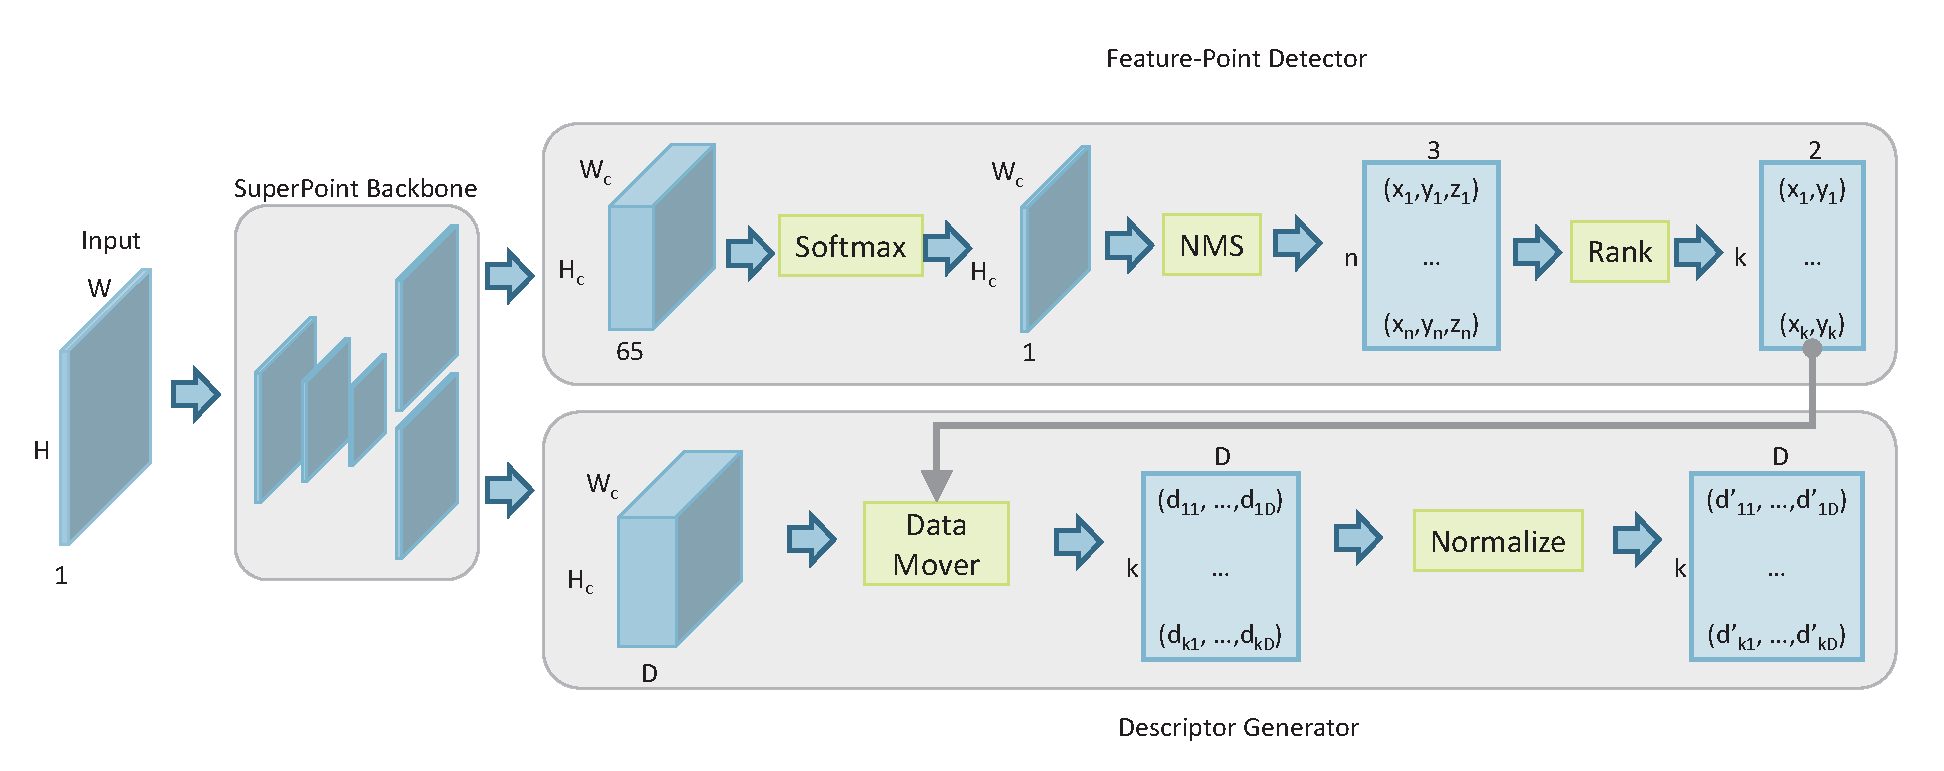
\includegraphics[width=0.95\linewidth]{fig/interexample.eps}
	\caption{ A simple example of accelerator interrupt based on Virtual Instruction. }
	\label{fig:interexample}
\end{figure*}

\subsubsection{ Virtual Filed}

Three values can be set to Virtual Filed:
\begin{itemize}
    \item[2'b00] indicates this instruction is not virtual, should always be executed.
    \item[2'b01] indicates this instruction is the SAVE instruction for backup. When an interrupt occurs, the high-priority network will start after this instruction.
    \item[2'b10] indicates this instruction is the LAOD instruction for recovery. The corresponding instructions will be executed after the high-priority network.
\end{itemize}

\subsubsection{ SaveID Filed }

SaveID links LAOD/CALC instructions to the corresponding SAVE instruction. SaveID of each not-virtual SAVE instruction differs. If the generated outputs of the LOAD/CALC are stored to DDR by a SAVE instruction, the LOAD/CALC instructions have the same SaveID as the SAVE instruction.

We consider all the LOAD/CALC instructions corresponding to one CALC\_F instruction as a \textbf{CalcBlob}. Each CalcBlob has one CALC\_F instruction, and ends up with this CALC\_F instruction. The SaveID for a CalcBlob is the same as its CALC\_F instruction.
One SAVE instruction may correspond to one CalcBlob ( \textbf{Single Blob Save}, illustrated in \Cref{fig:singlesave} ) or multiple CalcBlobs (\textbf{Multiple Blob Save}, illustrated in \Cref{fig:multisave}).

For Single Blob Save, no virtual SAVE is added. The high-priority network can be started after the nomal not-virtual SAVE. The virtual LOAD instructions for data recovery are generated after the normal SAVE, and executed after the high-priority network. The execution timeline is shown in \Cref{fig:intersinglesave}.

For Multiple Blob Save, virtual SAVE and LOAD instructions are generated after the CALC\_F of each CalcBlob. When the interrupt request occurs during the CalcBlob, the virtual SAVE instruction will be executed before the start of the high-priority network. Virtual LOAD instructions for data recovery are executed after the high-priority network. The subsequent nomal not-virtual SAVE instruction with the same SaveID as the CalcBlob will be modified to avoid duplicate output data transfer. The execution timeline is shown in \Cref{fig:intermultisave}.








\subsection{ Instruction Arrangement Unit (IAU) }

A specific hardware module called Instruction Arrangement Unit (IAU) is designed to handle the computing requirements from different tasks with different priorities. The IAU monitors the interrupt status, and generates a simple instruction sequence dynamically. The decoder, controller, processing elements in the CNN accelerator does not need to know the interrupt status, but only operate the instructions provided by IAU.

The hardware implementation of IAU is shown in \Cref{fig:IAU}, which supports four different tasks at different priorities. Task 0 has the highest priority and is uninterruptible. 

InstrAddr records the address to fetch the instructions of the corresponding task. The InputOffset and the OutputOffset are configured by the software, which indicate base address offsets of the input and output data. With the configuration of the offsets, low-latency ScratchPad memory \cite{Banakar2002Scratchpad} can be used for directly data sharing between CPU cores and accelerators. The data sharing with ScratchPad \cite{Banakar2002Scratchpad} is introduced in \Cref{sec:incame}.


SaveID, SaveAddr, and SaveLength record the backup status when an interrupt occurs. 
Subsequent not-virtual SAVE instructions will be modified according to the interrupt status recorded.
An example of the instruction modification will be given at \Cref{sec:exampleVirtual}.


\subsection{Example of Viutual Instruction}
\label{sec:exampleVirtual}


The example is based on a straightforward convolutional layer, which has only one input channel and one output channel. 
The convolution kernel size is $1 \times 1$. The shape of the input and output featuremaps is $ 2 \times 16 $ (\Cref{fig:interexample}(a) ). The two lines of output are calculated by two CALC\_F instructions ( instruction 3 and 7). The addresses used in the instruction example are listed in \Cref{fig:interexample}(b). \Cref{fig:interexample}(c) is the instruction sequence from DDR with virtual instructions. \Cref{fig:interexample}(d) is the executed instructions without interrupt. When an interrupt occurs at the first CACL\_F, \Cref{fig:interexample}(d) illustrated the backup and recovery instructions (Blue) and the modified SAVE instruction (Red).

% The hardware implementation of IAU is shouwn in \Cref{{fig:IAU}. There is a Status Pool which records the running states of each task. The InstrAddr is records the instruction address of each CNN

\section{Optimization For Post-Processing }
\label{sec:hardsoftcodesign}
\label{subsec:FEopt}

The high-priority feature-point extraction (FE) task is latency sensitive and needs to be computed before the next picture arrives. With the help of the CNN accelerator, the latency of CNN backbone is reduced with 30ms. However, the  post-processing of FE consumes 50+ms, which becomes the bottleneck of real-time feature-point extraction. In this section, the software and hardware acceleration for CNN-based Feature-point Extraction (FE) is introduced.


\begin{figure}[t]
    \centering  
    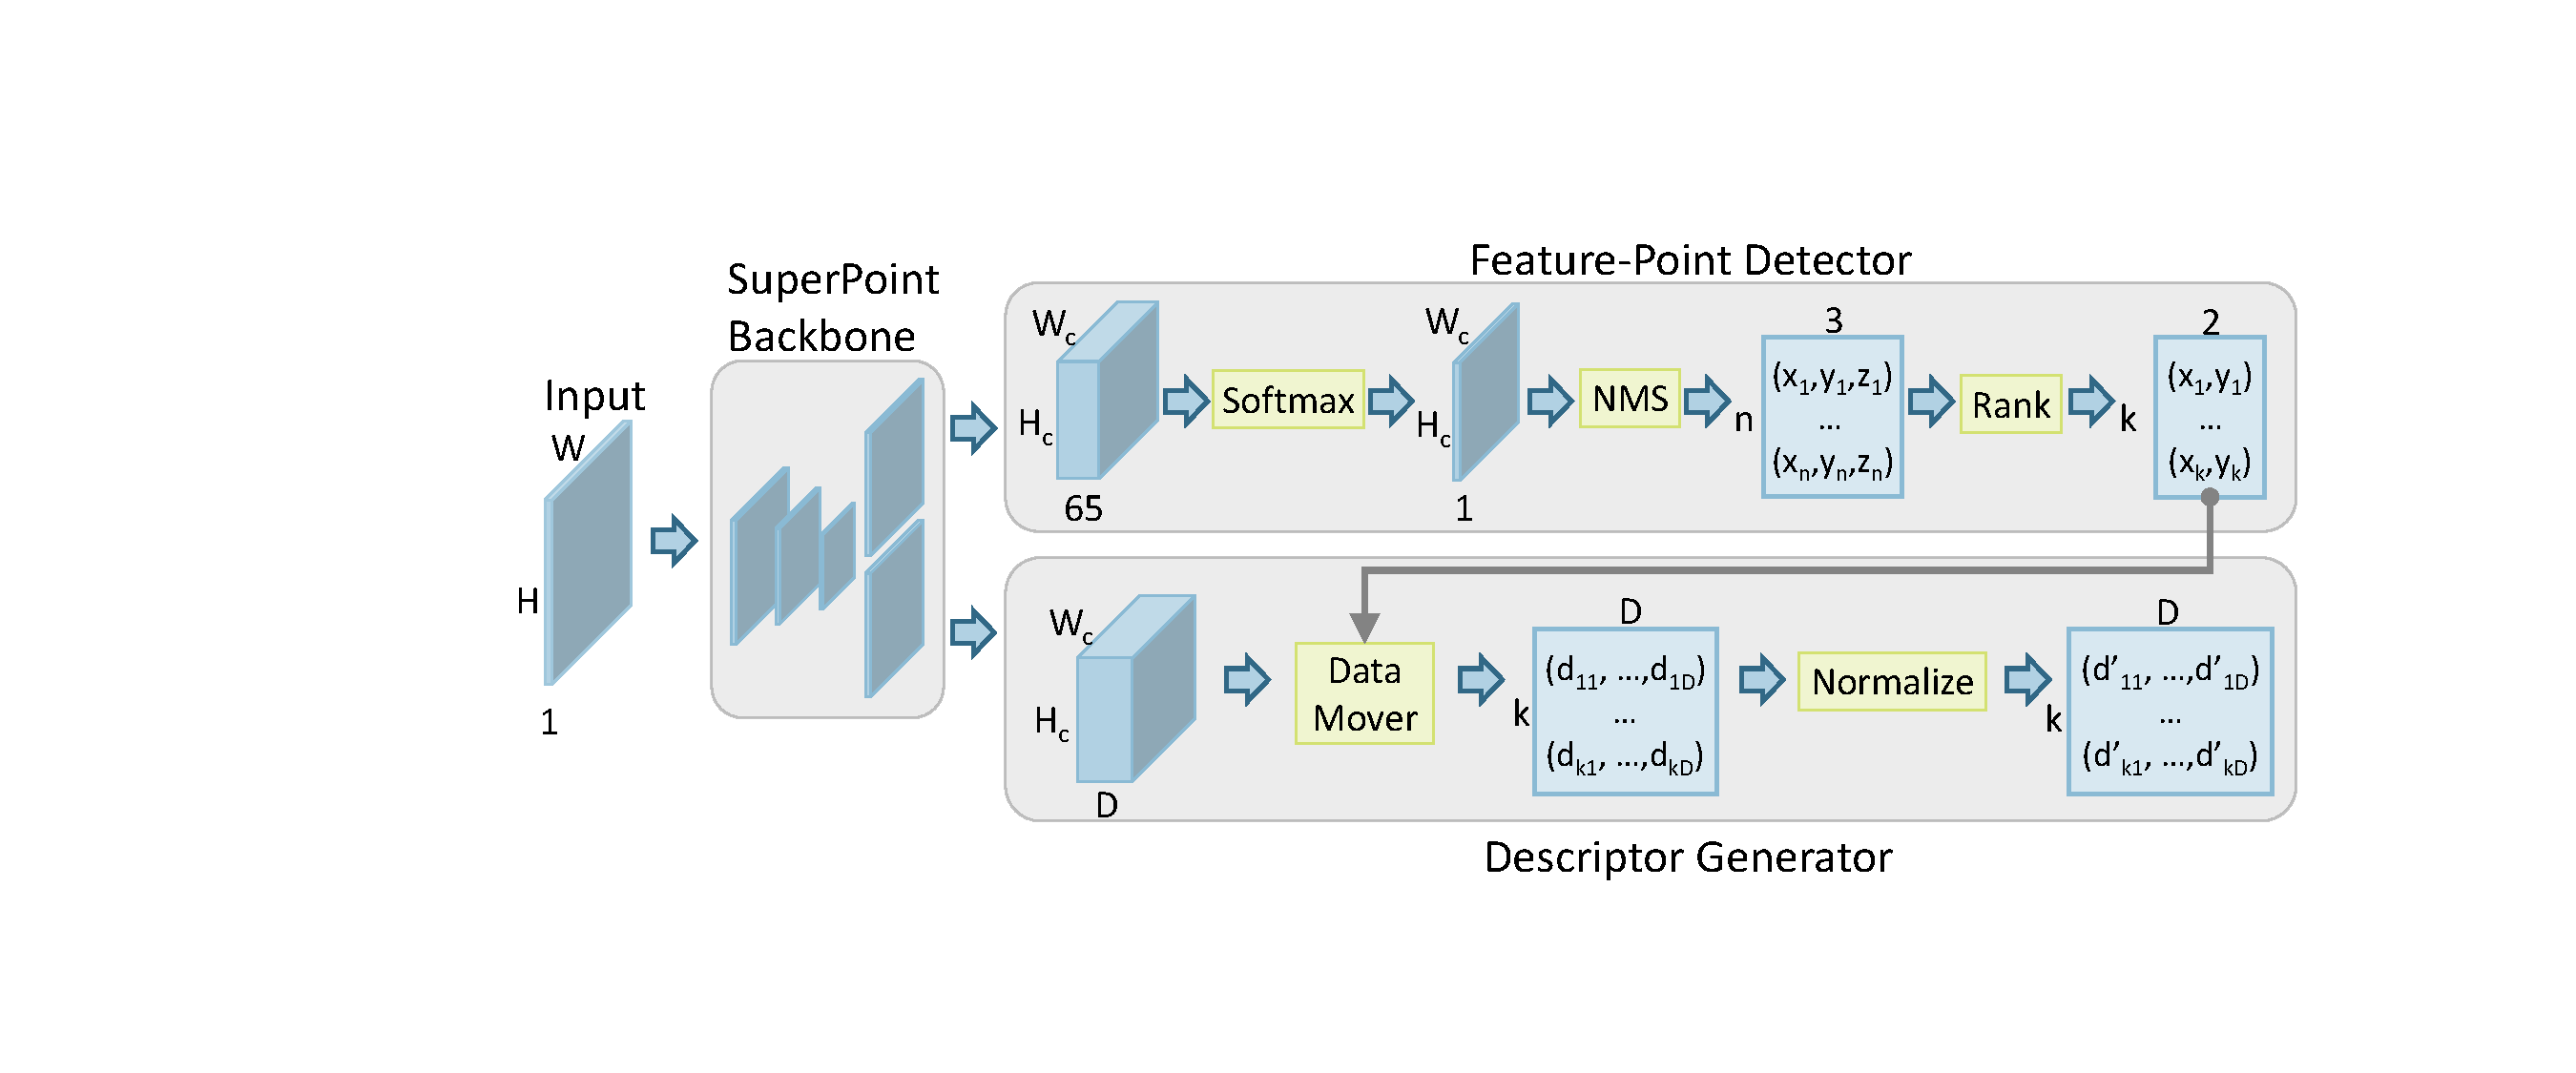
\includegraphics[width=1\linewidth]{fig/superpoint.pdf}
    \caption{Optimized feature extraction method based on SuperPoint}
    \label{fig:superpoint}
\end{figure}

As mentioned in \Cref{sec:relate}, there are two steps in the FE method: 1) feature-point detection and 2) feature descriptors generation. 
In SuperPoint \cite{detone2018superpoint}, there are three components in the feature-point detector, 1) Softmax to generate the confidence for each pixel, 2) Non-Maximum Suppression (NMS) to find the pixels with maximum confidence in its neighborhood, 3) Rank component to find out the first $k$ pixels with the highest confidence. 
In the feature descriptors step, the normalization component consumes most of the computation. 

The CNN backbone of SuperPoint maps the input image $I\in \mathbb{R}^{H\times W}$ to a tensor $\mathcal{X}\in \mathbb{R}^{H_c\times W_c\times 65}$ for feature-point detection and to a tensor $\mathcal{D}\in \mathbb{R}^{H_c\times W_c\times D}$ for descriptors generation, where $H_c = H/8$ and $W_c = W/8$.
We optimize the software data flow of the components above, making them less computationally complex and friendly to hardware. 
The flow path of our SuperPoint-based feature extraction method is shown \Cref{fig:superpoint}. 
Then we design FPGA accelerators specifically for calculating softmax and normalization.

\subsection{Softmax Optimization}
\label{sec:softmaxopt}

\begin{figure}[t]
    \centering  
    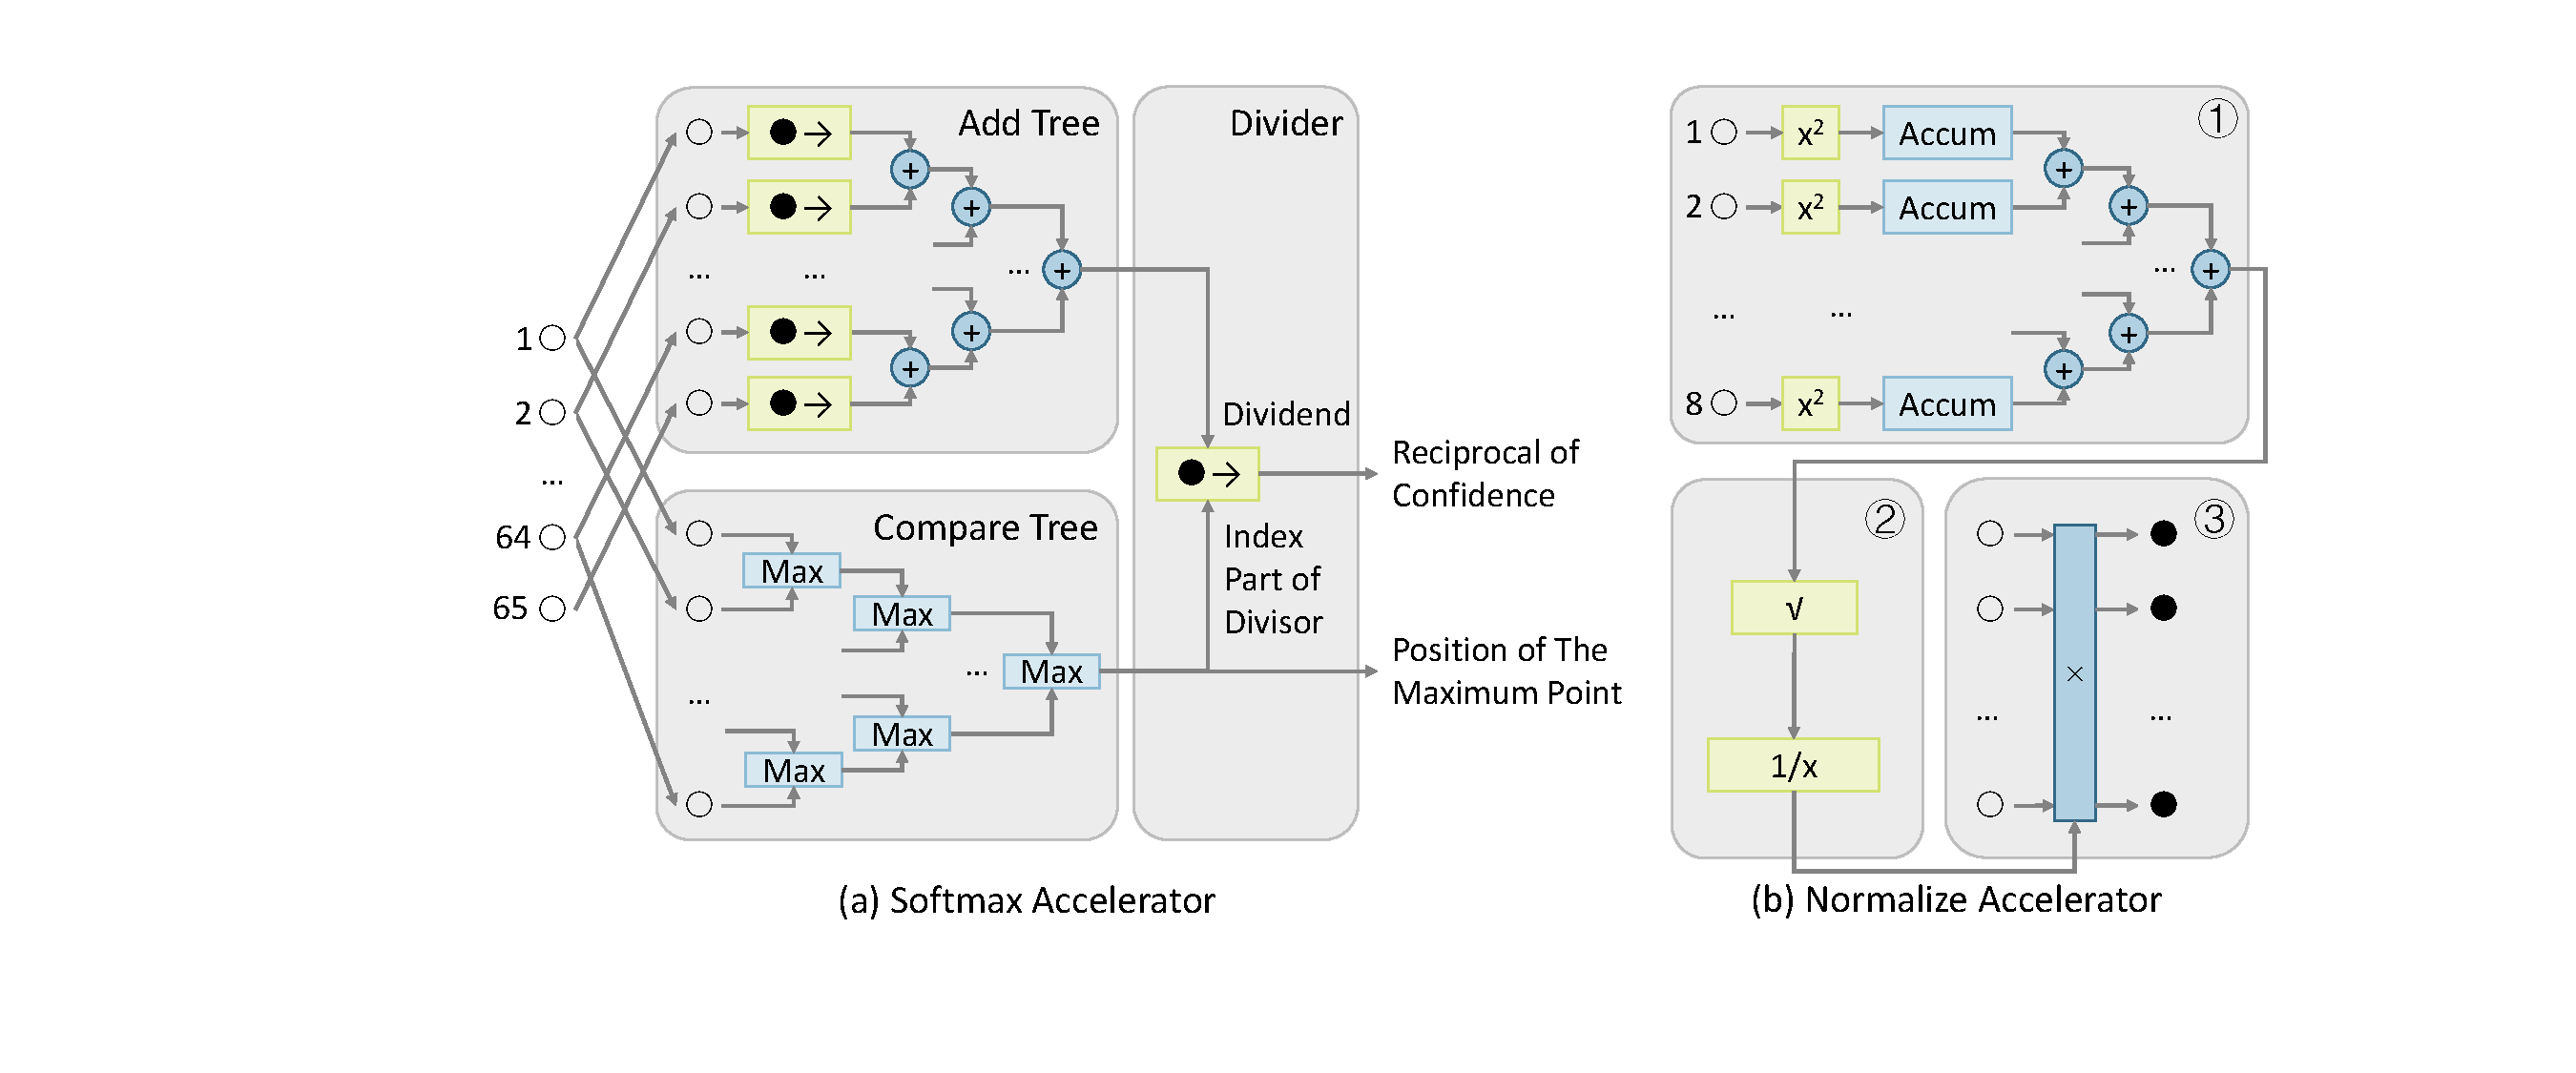
\includegraphics[width=1\linewidth]{fig/FEaccelerator.pdf}
    \caption{Hardware Architecture of FE Accelerators}
    \label{fig:FEaccelerator}
\end{figure}

For feature-point detection, the 65 channels correspond to local, non-overlapping $8 \times 8$ pixel grid areas plus a background channel. 
After a channel-wise softmax, the background channel is removed, and a $\mathbb{R}^{H_c\times W_c\times64}\Rightarrow \mathbb{R}^{H\times W}$ reshaping is performed. 
The channel-wise softmax makes the points in different grid areas have equal confidences.
The tensor of size $\mathbb{R}^{H\times W}$ corresponds to the confidences of the feature points in the input image.

The standard softmax function is defined as $\sigma (\mathbf {z} )_{i}$ in \Cref{equ:softmax_hard}.
We optimize the process of softmax that we only take the maximum value of each grid area for subsequent computations, which not only reduces the division operations of softmax but also simplifies the calculation of NMS and Rank.
We reduce the division operations and output size of softmax from $H \times W$ to $H_c \times W_c$.
The division operation is resource consuming on FPGA platforms. 
Our method can greatly reduce the number of divisions by $64 \times$, making it easy to accelerate softmax operation on FPGA.

\begin{equation}
    \sigma (\mathbf {z} )_{i}={\frac {e^{z_{i}}}{\sum _{j=1}^{K}e^{z_{j}}}}
    \Rightarrow
    \frac{1}{\sigma (\mathbf {z} )_{i}}={\frac {\sum _{j=1}^{K}2^{z_{j}}}{2^{z_{i}}}}{\text{ for }}i=1,\dotsc ,64;
    \label{equ:softmax_hard}
\end{equation}

Since the results of the softmax function are all positive, we can calculate the reciprocal of the softmax function ($\frac{1}{\sigma (\mathbf {z} )_{i}}$) in \Cref{equ:softmax_hard} as the normalized confidence, without affecting the results of the NMS and ranking process. We quantize the output feature map of CNN to 8-bit fixed-point integer, i.e each $z_i$ in \Cref{equ:softmax_hard} is a 8-bit fixed-point integer. We change the base of the power from $e$ to $2$ to make it hardware friendly. Since the divisor is a power of $2$, we can also implement division by shift operation.

\Cref{fig:FEaccelerator}(a) shows an overview of the softmax module. It consists of three parts, add tree, compare tree and divider. Softmax reads 65 numbers from a grid region at once. Add tree computes input to the power of $2$ using shift operation and calculates their sum. Compare tree reads the values of the first 64 channels and returns the maximum value and its channel number which contains position information. The divider uses the shift operation to calculate the reciprocal of confidence.

\subsection{NMS Optimization}

Non-maximum suppression(NMS) is applied to the detection to help ensure that the feature-points are evenly distributed throughout the image. 
For each pixel in the original input image, NMS compares the confidence of this pixel with that of the pixels in a square neighborhood whose edge including $\epsilon _{ori}$ pixels. 
If the confidence of the target central pixel is not the maximum in its neighbors, this point will be eliminated from the valid feature-points. 
The output of the NMS is a list of coordinates and confidences for each feature-point. 
There are totally $H \times W$ points and the NMS does $\epsilon _{ori} ^ 2 - 1$ comparison operations for each points. 
Thus, in the original NMS method, there are totally $H \times W \times (\epsilon _{ori} ^ 2 - 1)$ comparison operations.

The softmax optimization introduced in \Cref{sec:softmaxopt} already gives the pixel with maximum confidence of each $8 \times 8$ block. Thus, we only need to compare each output pixel of softmax to the its adjacent blocks. The comparison area is a square box with an edge of $\epsilon _{opt}$ pixels. and $\epsilon _{opt} = 2\times \left \lceil (\epsilon _{ori}-1)/16 \right \rceil +1$. There are only $H_c \times W_c$ points. Thus, after NMS optimization, there are totally $H_c \times W_c \times (\epsilon _{opt} ^ 2 - 1)$ comparison operations.

The $\epsilon _{ori}$ is set to 9 in the original implements SuperPoint, so $\epsilon _{opt} = 2\times \left \lceil (\epsilon _{ori}-1)/16 \right \rceil +1 = 3$. So that $H \times W \times 80 $ comparisons are done in the original NMS and we can do only $H_c \times W_c \times 8$ comparisons after optimization. The total number of comparisons is reduced by $640\times$.

\subsection{Ranking Optimization}

The ranking operation is to find out the top $k$ feature-points with maximum confidence. 
The output is a list of coordinates for the $k$ feature-points. 
In the original implementation, the confidence of all valid feature-points after NMS is sorted, and only the first $k$ feature points are used in the applications like SLAM and image matching. 
There are $N_{nms}$ valid points after NMS. To sort all these $N_{nms}$ points, the time complexity is defined as:

\begin{equation}
    C_{sort} = O(N_{nms} \cdot log(N_{nms}))
    \label{equ:csort}
\end{equation}

We create a heap of size $k$ and then look for the $k$ feature-points with the highest confidence. We do not compute the order of these $k$ points. The time complexity of the optimized ranking method is:

\begin{equation}
    C_{heap} = O(N_{nms} \cdot log(k))
    \label{equ:optsort}
\end{equation}

In our expetiments, $N_{nms} \approx 2000$ and $k = 200$. The number of comparisons is reduced by $1.4\times$.

\subsection{Normalization Optimization}

The input of the descriptor head sized $\mathbb{R}^{H_c\times W_c\times D}$ is semi-dense descriptor that each $8\times8$ pixel cell has a descriptor. In the original implementation, a bicubic interpolation and normalization yields fine descriptors of size $\mathbb{R}^{H\times W\times D}$. Then, according to the result of the rank, the descriptors corresponding to the k feature points are combined into a list and output. When using maximum point softmax, each $8\times8$ pixel cell only has a potential feature-point. So we can use semi-dense descriptor as the dense descriptor of the potential feature-point and do not need bi-cubic interpolation.

The number of descriptors that need to be normalized has been reduced from $H\times W$ to $H_c\times W_c$. In addition, we normalize the descriptors after sorting the feature-points, which means we only need to normalize $k$ descriptors. If we set $H=480$, $W=640$ and $k=200$, then the computational complexity of the normalization process will be reduced by $1500\times$. However, $k$ descriptors are not stored in contiguous memory space. We use a datamover to move data from discrete address spaces.

The architecture of normalization accelerator is illustrated in \Cref{fig:FEaccelerator}(b). The normalization module can read 8 numbers per clock cycle. The normalization process is divided into three stages and requires each descriptor to be read twice. In the first stage, we compute the sum of the squares of the descriptors, which takes 32 clock cycles when $D=256$. Then the reciprocal of square root of sum is computed as the normalization coefficient. In the final stage, the descriptor is read a second time and multiplied by the normalization coefficient.

% \subsection{Optimization for PR Post-Processing}

% \begin{figure}[t]
%     \centering
%     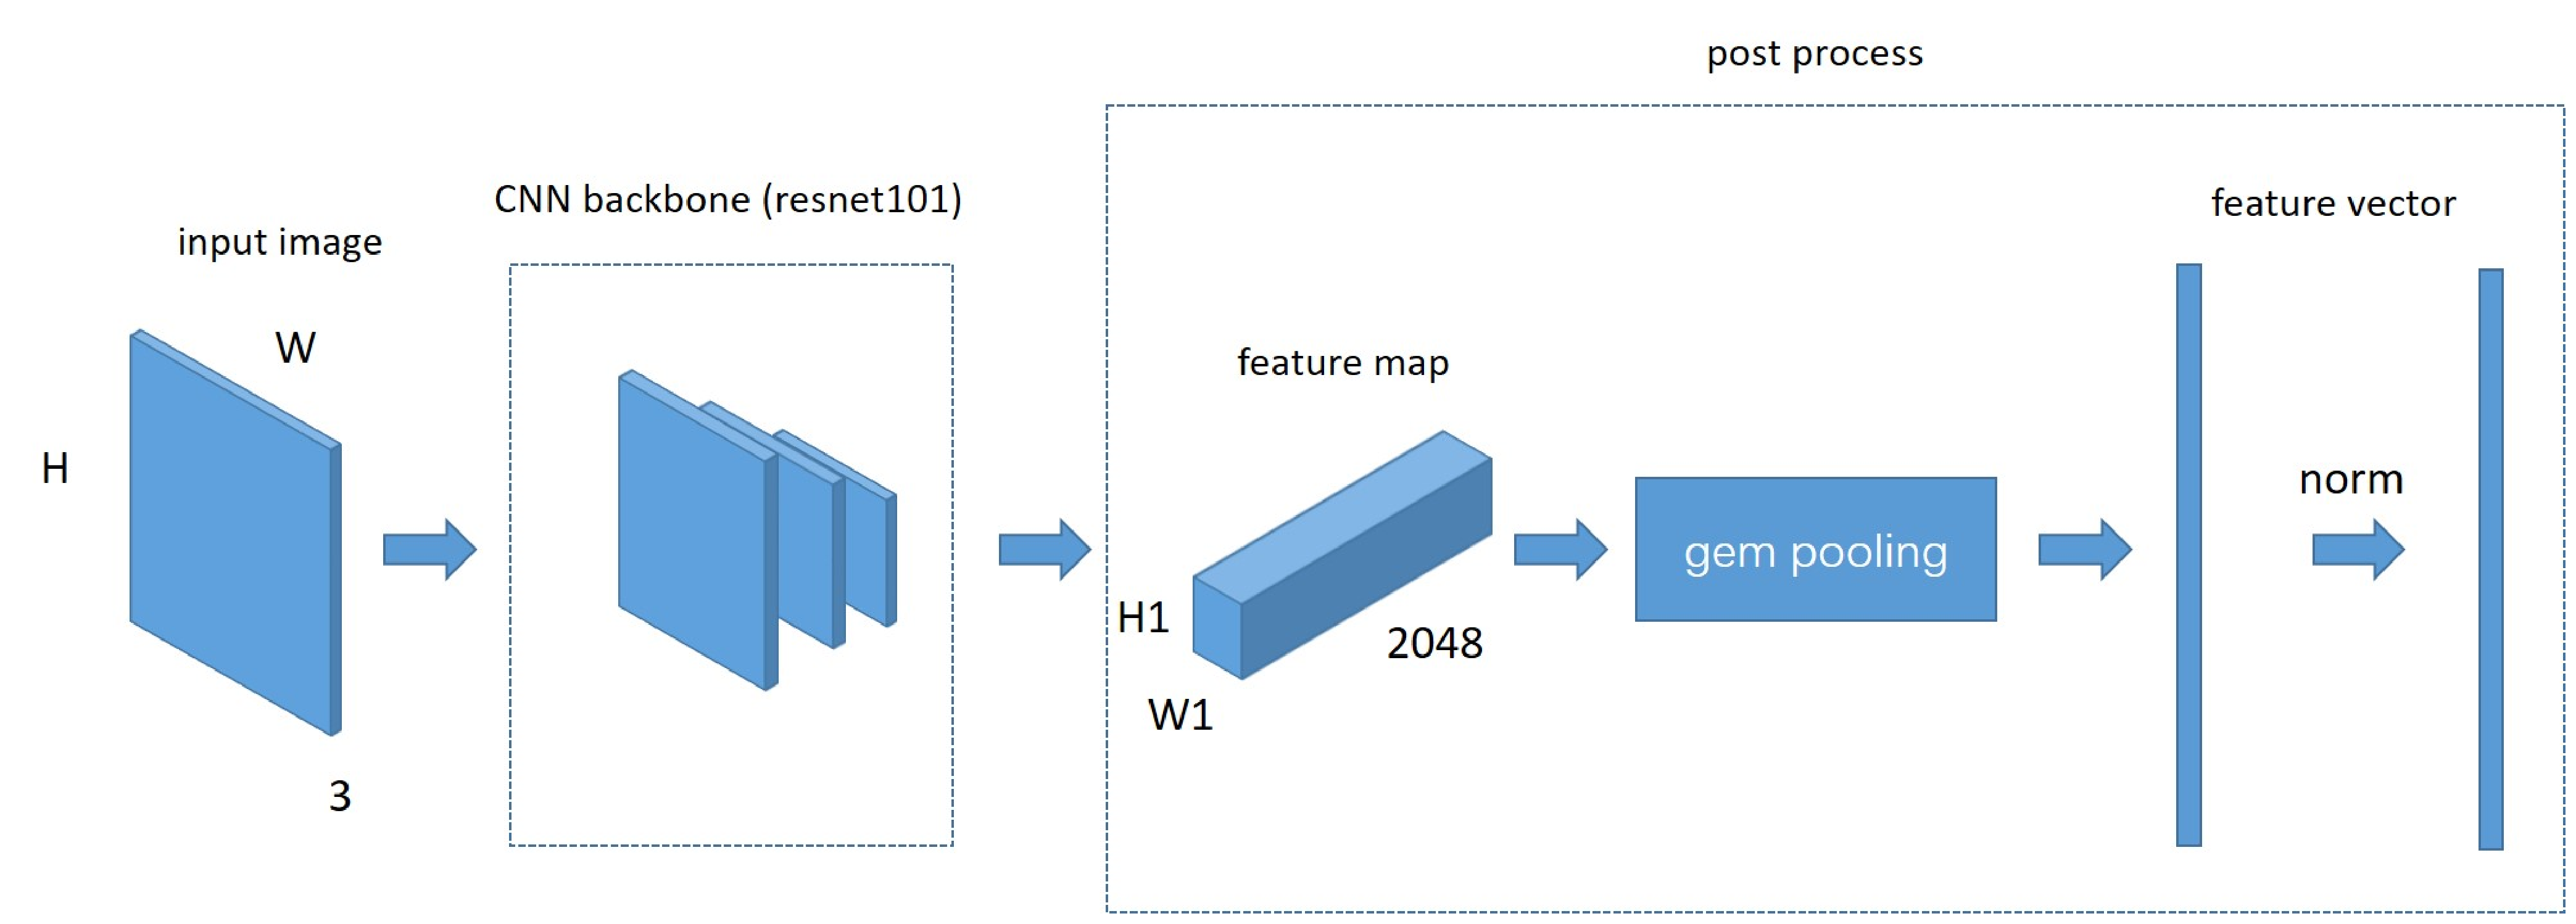
\includegraphics[width=1\linewidth]{fig/pr.eps}
%     \caption{The architecture of GeM network}
%     \label{fig:gem}
% \end{figure}

% Figure \ref{fig:gem} shows the data flow of GeM network \cite{gem} for PR. The CNN backbone of GeM is a resnet101 network without the last two layers(pooling and FC). The CNN maps the input image $ I \in \mathbb{R}^{3 \times H \times W}$ to a tensor $\mathcal{X} \in \mathbb{R}^{C \times H_1 \times W_1}$. Here, the channel number $C = 2048$. Then the gem pooling layer pool the tensor into a vector $\mathcal{V} \in \mathbb{R}^{C}$. (To avoid ambiguity, we use "GeM" to represent the whole network and "gem" to represent the pooling layer only.) Finally, the vector is normalized. After that, we use dot product or L2 distance of the vectors to calculate similarity of places. Because feature extraction needs to be real-time and is time consuming, we modify its software utilization and design FPGA accelertor for this process.

% Experiments show that the post processing (gem pooling and normalization) consume nearly twice the time as CNN network does. After optimization, we can reduce time to 1/? of that of origin.

% \subsubsection{GeM Pooling Optimization}

% The element of the vector $\mathcal{V}$ is calculated by

% \begin{equation}
%     \mathcal{V}_i = (\sum_{x \in \mathcal{C}_i} x^p)^{1/p}, i=1, 2, ..., 2048.
% \end{equation}

% Here, the parameter $p$ is learned by back propagation and is set to 2.9? in original paper. To make it friendly for hardware computation, we change it to $p=3$. In this way, the power computation can be converted to multiplication computation. This will save a lot of time and calculation resources on FPGA without loss of accuracy. We notice that the channels are independent with each other, so it's convenient to do parallel computation on FPGA. With Vivado HLS tool, we design an IP core for gem pooling and efficiently reduce time.

% \subsubsection{Normalization Optimization}

\section{Evaluation and Results}
\label{sec:experiments}

In this section, the evaluation of the instruction-based-interruption, hardware modules for post-processing, and the overall MA-Explore system are presented and analyzed.

\subsection{ Instruction-based-interruption}

The proposed interruptible is implemented and evaluated on the Xilinx ZCU102 evaluation board \cite{zcu102}. The CNN accelerator is developed based on the Xilinx AI accelerator, DPU \cite{dpu}. 

% The performance and the latency of the interruptible DPU and the not-interruptible DPU are listed in \Cref{tab:anywhere}. 
In MR-Explore, only the low-priority PR task is interruptible, and the interrupt position is unpredictable.
We record some of the interrupt locations when running MR-Explore on the interruptible DPU. The performance and the latency of the interruptible DPU and the not-interruptible DPU are listed in \Cref{tab:anywhere}. 
The execution time (Exe time) in \Cref{tab:anywhere} shows the time to complete two tasks, a interruptible PR task and a FE task.

The 'Serial' row is the baseline for executing the two tasks in serial. In serial execution, backup/recovery of data is not required. The 'CPU-like' row is the estimated result of backup/recovery all the on-chip caches for immediately interruption. The 'Pose 1,2,3' rows are the results of the DPU interrupted at different  PR positions. 'Pose 1' represents the first layers of PR network, the numbers of input channel and output channel are both $64$. The input and output shapes are both $240 \times 320$. 'Pose 2' represents the layers with moderate number of channels ($ 512 $) and data shapes ($ 60 \times 80 $). 'Pose 3' represents the last layers with many channels ($ 2048 $) and small featuremaps ($ 15 \times 20$).

DPU first calculates all channels of the output row before calculating the next rows. As the number of channels increases, the number of weights requiring recovery increases squarely. However, the size of the input data to be restored and the output results to be backed up remains basically the same.


% Table generated by Excel2LaTeX from sheet 'Sheet2'
\begin{table}[t]
  \small
  \centering
  \caption{Pref. for different interrupt positions.}
    % Table generated by Excel2LaTeX from sheet 'Sheet2'
\begin{tabular}{|c|c|c|c|c|c|}
  \hline
        & Backup  & Recovery & Exe time & Perf. & Latency \bigstrut[t]\\
        & (KB)  & (KB)  & (ms)  & Reduce & (ms) \bigstrut[b]\\
  \hline
  Pose 1 &       &       &       &       &  \bigstrut\\
  \hline
  Pose 2 &       &       &       &       &  \bigstrut\\
  \hline
  Pose 3 &       &       &       &       &  \bigstrut\\
  \hline
  CPU-Like & 4000  & 4000  &       &       & <1 \bigstrut\\
  \hline
  Serial & -     & -     &       &  baseline & - \bigstrut\\
  \hline
  \end{tabular}%
  
  
  \label{tab:anywhere}%
\end{table}%



% % Table generated by Excel2LaTeX from sheet 'Sheet1'
% \begin{table}[t]
%     \centering
%     \caption{Interrupt after complete results vs Interrupt anywhere}
% % Table generated by Excel2LaTeX from sheet 'Sheet2'
% \begin{tabular}{|c|c|c|c|c|c|}
%   \hline
%   \multicolumn{1}{|c}{} &       & \multicolumn{1}{c|}{Backup } & \multicolumn{1}{c|}{Recovery} & Exe time & Performance \bigstrut[t]\\
%   \multicolumn{1}{|c}{} &       & \multicolumn{1}{c|}{data (KB)} & \multicolumn{1}{c|}{ data (KB)} & (ms)  & Reduce \bigstrut[b]\\
%   \hline
%   \multicolumn{1}{|p{3.315em}|}{Inter } & \multicolumn{1}{p{3.69em}|}{AfterSave} &       &       &       &  \bigstrut\\
%   \cline{2-6}\multicolumn{1}{|p{3.315em}|}{position 1} & Anyware &       &       &       &  \bigstrut\\
%   \hline
%   \multicolumn{1}{|p{3.315em}|}{Inter } & \multicolumn{1}{p{3.69em}|}{AfterSave} &       &       &       &  \bigstrut\\
%   \cline{2-6}\multicolumn{1}{|p{3.315em}|}{ position 2} & Anyware &       &       &       &  \bigstrut\\
%   \hline
%   \multicolumn{1}{|p{3.315em}|}{Inter } & \multicolumn{1}{p{3.69em}|}{AfterSave} &       &       &       &  \bigstrut\\
%   \cline{2-6}\multicolumn{1}{|p{3.315em}|}{position 3} & Anyware &       &       &       &  \bigstrut\\
%   \hline
%   \multicolumn{2}{|p{7.005em}|}{CPU-Like} &       &       &       &  \bigstrut\\
%   \hline
%   \multicolumn{1}{|c}{} &       & \multicolumn{1}{c|}{Instruction} & \multicolumn{1}{c|}{Latency} & Exe time & Performance \bigstrut[t]\\
%   \multicolumn{1}{|c}{} &       & \multicolumn{1}{c|}{ (KB)} & \multicolumn{1}{c|}{(ms)} & (ms)  & Reduce \bigstrut[b]\\
%   \hline
%   \multicolumn{1}{|c|}{No} & \multicolumn{1}{p{3.69em}|}{Origin} &       &       &       & 0 \bigstrut\\
%   \cline{2-6}\multicolumn{1}{|c|}{ Interrupt} & \multicolumn{1}{p{3.69em}|}{After results} &       &       &       &  \bigstrut\\
%   \cline{2-6}      & Anyware &       &       &       &  \bigstrut\\
%   \hline
%   \end{tabular}%
  
%     \label{tab:anywhere}%
%   \end{table}%



\subsection{ Place Recognition With DPU }

In this section, we design experiments to evaluate the accuracy and efficiency of the PR network on DPU. 

\subsubsection{accuracy}

\begin{figure}[ht]
    \centering
    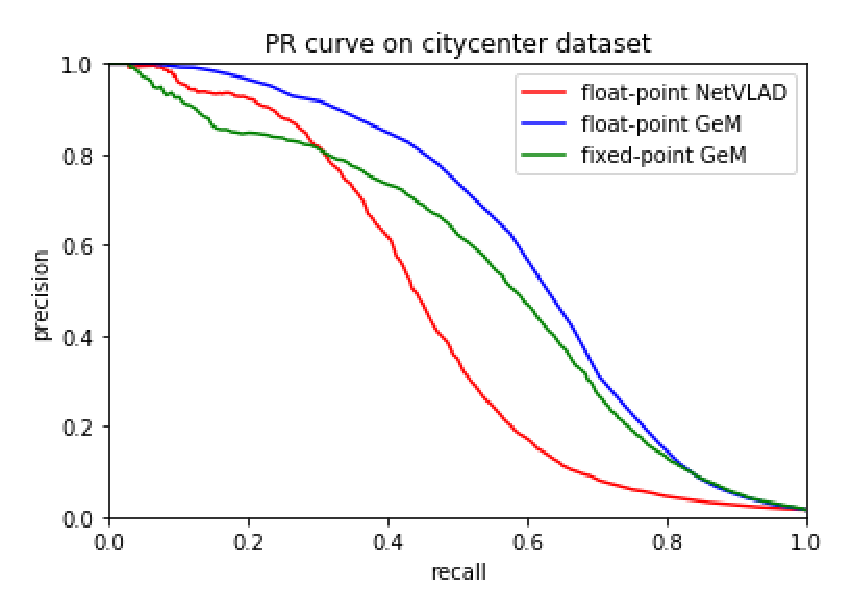
\includegraphics[width=0.8\linewidth]{fig/result.eps}
    \caption{Precision-Recall curve on Citycenter dataset}
    \label{fig:PRcurve}
\end{figure}

We want to prove two things in our experiment. 1) The GeM network used in our work outperforms other networks such as NetVLAD. 2) The quantization of GeM CNN backbone don't bring about much drop in accuracy. We test 3 networks, a) float-point GeM, b) float-point NetVLAD, c) fixed-point GeM on Citycenter dataset and draw the Precision-Recall curve. The result is shown in figure \ref{fig:PRcurve}. It's clear that float-point GeM netowrk run better than NetVLAD in all situations. After quantization, the accuracy goes down a bit, especially when precision is high. But the quantized network still outperforms NetVLAD in most cases.

\begin{figure}[ht]
  \centering
  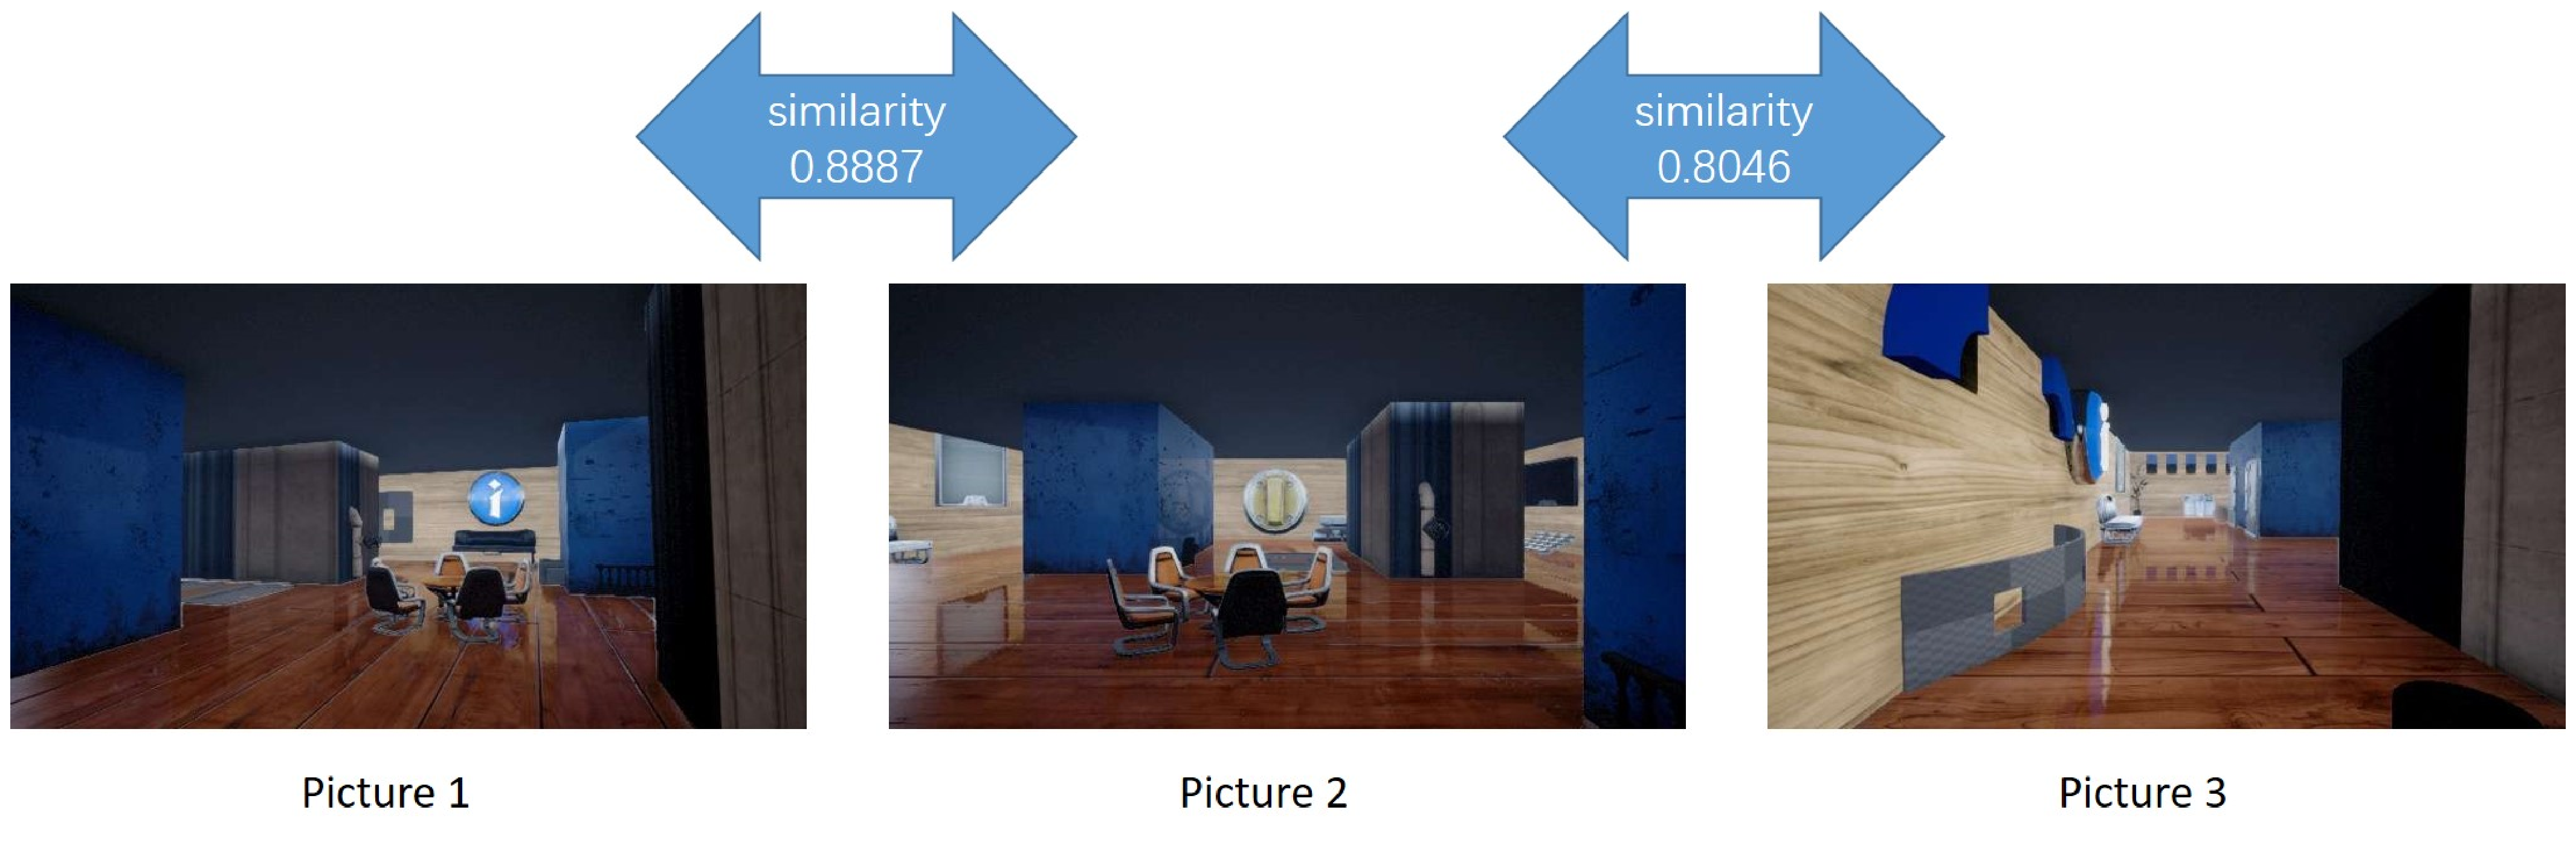
\includegraphics[width=0.8\linewidth]{fig/example.eps}
  \caption{Example of GeM performance.}
  \label{fig:gem_exp}
\end{figure}

Figure \ref{fig:gem_exp} shows an example in our similation environment. Picture 1 and Picture 2 is photoed in the same place and Picture 3 is photoed in another place. The computed similarity of Picture 1 and 2 is 0.8887, apparently larger than the similarity of Picture 2 and 3 (0.8046).

\subsubsection{efficiency}

\begin{table}
    \label{tab:gem_eff}
    \centering 
    \caption{runtime comparison of each operation in PR}
    \begin{tabular}{|c|c|c|}
				\hline
              & CPU & CPU+FPGA \\
        \hline
           &   48 ms &   42 ms \\
			  \hline
    \end{tabular}
  \end{table}

As illustrated in section \ref{sec:hardsoftcodesign}, we do optimization on GeM backend processing, i.e., the gem pooling layer. We compare running time before and after optimization, and the result is shown in table \ref{tab:gem_eff}. After optimization, the total time reduces by 12.5\%.


\subsection{ VO With DPU }

To evaluate the performance of the SuperPoint network in visual odometer, we experimented on the $TUM$ dataset. We evaluate SuperPoint against two well-known FE systems: SIFT\cite{Lowe-478} and ORB\cite{RubleeRabaud-479}. We apply the three systems to the visual odometer. We also evaluate the performance after optimization. We compute a maximum of 200 points for all systems at a $480\times640$ resolution and set $NMS=4$. We perform nearest neighbor matching from descriptors in adjacent frames with a maximum allowable distance $d_m$. $d_m$ is not same in three system because descriptors are not in the same order of magnitude. We use an OpenCV implementation (solvePnP()) with all the matches to compute the transform matrix, and use Bundle Adjustment to optimize results. All the computation of this experiment is all done on the CPU except CNN of SuperPoint. 

\begin{table}[t]
  \centering
  \caption{ Accuracy and runtime results on the TUM\cite{sturm12iros} SLAM dataset  }
  \footnotesize
  \begin{threeparttable}
% Table generated by Excel2LaTeX from sheet 'Sheet2'
\begin{tabular}{|c|c|c|c|c|} 
  \hline
        & \multirow{2}[2]{*}{$d_m$$^1$} & RPE$^2$ & ATE$^3$  & Run  \bigstrut[t]\\
        &       &  (m/s) & (m) & time(ms) \bigstrut[b]\\
  \hline
  SIFT  & 200   & 0.0319  & 0.4219 & 2397  \bigstrut\\
  \hline
  ORB   & 30    & 0.0577  & 0.6105 & 229  \bigstrut\\
  \hline
  Origin & \multirow{2}[2]{*}{0.7} & \multirow{2}[2]{*}{0.0280} & \multirow{2}[2]{*}{0.3671} & \multirow{2}[2]{*}{259} \bigstrut[t]\\
   Superpoint &       &       &       &  \bigstrut[b]\\
  \hline
  Our Fixed & \multirow{2}[2]{*}{360} & \multirow{2}[2]{*}{0.0283} & \multirow{2}[2]{*}{0.3976} & \multirow{2}[2]{*}{59} \bigstrut[t]\\
   Superpoint &       &       &       &  \bigstrut[b]\\
  \hline
  \end{tabular}%
  

\begin{tablenotes}
  \item[1] $d_m$ is the maximum allowable distance between matched descriptors.  
  \item[2] RPE is the mean Relative Pose Error to indicate the translational drift per second, the less, the better.
  \item[3] ATE is the root mean square Absolute Trajectory Error to indicate the translational drift of the entire trajectory, the less, the better.
\end{tablenotes}
    \end{threeparttable}
  \label{tab:VO}%
\end{table}%

Results are shown in \Cref{tab:VO}. In terms of accuracy, SuperPoint outperforms ORB and performs comparably to SIFT. Optimization does not introduce a large loss of accuracy. In terms of calculation speed, SuperPoint takes less time than Sift, and is equivalent to Orb. After optimization, the running speed is increased by $4\times$, making real-time processing possible.

\begin{table}[t]
  \centering
  \caption{runtime Comparison of each operation}
% Table generated by Excel2LaTeX from sheet 'Sheet2'
\begin{tabular}{|c|c|c|c|c|}
  \hline
             &    softmax &        NMS &       rank &  normalize \bigstrut\\
  \hline
         CPU &       31ms &       27ms &       0.97ms &       42ms \bigstrut\\
  \hline
    CPU+FPGA &     1.97ms &      0.7ms &     0.12ms &     1.44ms \bigstrut\\
  \hline
  \end{tabular}  
  
  \label{tab:optimization}%
\end{table}%

We compare the running time of each operation in SuperPoint before and after the optimization. Results are shown in \Cref{tab:optimization}. The running time of each operation is reduced by more than $20\times$. There is a certain gap between the experimental results of the acceleration effect and the theoretical derivation in \Cref{subsec:FEopt}. The possible reason is that the CPU needs time to schedule the FPGA accelerator.

\subsection{ ROS based MA-Explore }

\subsubsection { Hardware Resources Utilization }

The proposed ROS based MA-Explore is inplemented and evaluated on the ZCU102 evaluate board \cite{zcu102}, which is provied by Xilinx. The CNN backbone is calculated by Xilinx AI accelerator, DPU\cite{dpu}, which is a hardware IP implemented on the FPGA side of ZCU102 (Programable logic, PL side). The FE and the PR post-processing steps run on our proposed accelerators, also on the PL side. The PL side has 3 clock frequencies. The DPU are running at 300MHz. The accelerator for FE are running at 200MHz and the accelerator for PR are running at 100MHz.

\Cref{tab:hardware} shows the hardware resources utilization of DPU and our proposed accelerators. About 48\% of on-board hardware resources are used by DPU. Our proposed accelerators only use a small amount of hardware resources compared with the DPU.
% Table generated by Excel2LaTeX from sheet 'Sheet1'
\begin{table}[t]
  \centering
  \caption{Hardware comsumption of the proposed hardware}
% Table generated by Excel2LaTeX from sheet 'Sheet1'
\begin{tabular}{|c|c|c|c|c|}
  \hline
        & $\sharp$ DSP & $\sharp$ LUT & $\sharp$ FF & $\sharp$ BRAM \bigstrut\\
  \hline
  On-Board Resource &   2520   &  274080      &  548160     & 912 \bigstrut\\
  \hline
  DPU &   1282   &  74569      &   171416    & 499 \bigstrut\\
  \hline
  FE & 25      &  17573     &   29115    & 10 \bigstrut\\
  \hline
  PR & 109      &  7169     &   5601    & 11.5 \bigstrut\\
  \hline
  \end{tabular}%
  
  
  
  
  \label{tab:hardware}%
\end{table}%

\section{Conclusion}
\label{sec:conclusion}

We propose an interruptible CBN accelerator for multi-agent exploration.

%%
%% The acknowledgments section is defined using the "acks" environment
%% (and NOT an unnumbered section). This ensures the proper
%% identification of the section in the article metadata, and the
%% consistent spelling of the heading.
% \begin{acks}
% To Robert, for the bagels and explaining CMYK and color spaces.
% \end{acks}

%%
%% The next two lines define the bibliography style to be used, and
%% the bibliography file.
\bibliographystyle{ACM-Reference-Format}
\bibliography{src/fpgaslam}

%%
%% If your work has an appendix, this is the place to put it.
% \appendix

\end{document}
\endinput
%%
%% End of file `sample-sigconf.tex'.
